
\section{Fundamental quantum algorithms}
\label{high_level_algo_summary}

In this section we summarize quantum algorithms that can be used for materials science applications. We consider algorithms that simulate quantum systems and mention quantum computing approaches to simulate partial differential equations (PDEs). Although the simulation of quantum systems is the most natural application of quantum computers in the materials science space, we mention  quantum algorithms for PDEs since they can be useful for some well-crafted use cases. Within the simulation category, we discuss the time dynamics, ground states, open quantum systems and finite-temperature properties. 

Simulation of dynamics generated by a Hamiltonian of interest is one of the most natural applications for quantum computers.
Quantum algorithms for approximating time evolution have been studied extensively, and we just name a few key methods here.
In recent years the development of \emph{quantum signal processing} culminated in an algorithm called \emph{qubitization}~\cite{low2019hamiltonian}, the complexity of which is measured by the number of queries to an oracle that encodes the Hamiltonian.
For a target evolution time $t$ and an error tolerance $\epsilon$, qubitization makes only $O(t + \log 1/\epsilon)$ queries to the oracle, which is asymptotically optimal. However, the construction of the Hamiltonian oracle generally involves ancillary qubits, making qubitization difficult to implement in near-term and early fault-tolerant devices. 

In this regime, \emph{Trotterization}~\cite{lloyd1996universal,childs2019theory} (see also Sec.~\ref{trotter_sec}), despite being the original quantum algorithm for simulating dynamics, remains one of the leading candidates for early applications, because its low overhead permits fine-grained tradeoffs between circuit depth and accuracy.
Asymptotically, the gate complexity of the $p$-th order Trotterization scales as $O(t^{1+1/p}/\epsilon^{1/p})$, which can be made close to that of qubitization at large $p$.
Additionally, the error of Trotterization depends on the commutativity of the terms in the Hamiltonian, allowing the algorithm to take advantage of the structure of the Hamiltonian.
The final example we mention is the \emph{HHKL} algorithm~\cite{hhkl2018}, which achieves nearly optimal scalings for Hamiltonians that are geometrically local (or even with power-law decaying interactions~\cite{tran2019locality}) on some lattice.
HHKL can be considered a hybrid between Trotterization and the high-accuracy methods that exploits commutation between spatially-separated Hamiltonian terms.

Perhaps the most paradigmatic type of quantum simulation for materials is the approximation of ground states and low-energy states in general.
While such problems are QMA-hard~\cite{kitaev02,kempekitaevregev04} and thus believed to be intractable in worst cases, their broad utility across physics, chemistry, and materials science has made them the objects of intense study in the hope that for physically interesting cases, they may be manageable.
The most heavily studied algorithm for simulating ground states in the near term is the \emph{variational quantum eigensolver} (VQE, e.g.,~\cite{du2010nmr,lanyon2010towards,peruzzo2014variational,wang2015quantum,omalley2016scalable,shen2017quantum,paesani2017bayesian,kandala2017hardware,hempel2018trappedion,santagati2018witnessing,dumitrescu2018atomicnucleus,kokail2019selfverifying,kandala2019errormitigation,ganzhorn2019gate,sagastizabal2019experimental,mccaskey2019quantum,smart2019quantum,nam2020trappedion,liu2021representation,wang2021resource,liu2023analytic,zheng2023speeding,wang2023ever}), which is based on optimizing a parameterized wavefunction prepared on the quantum computer, and is well-adapted to near term due to the possibility of implementing it with low-depth circuits. Similar considerations apply to the use of finite-depth quantum approximate optimization algorithms for finding the ground state of frustrated materials \cite{doi:10.1073/pnas.2006373117,lotshaw2023simulations}.
However, VQE has a number of drawbacks, mostly related to the difficulties of establishing convergence of the optimization and of accurately measuring the target energy to be estimated, which can result in long runtimes or getting stuck in local minima. 

If we consider fault-tolerant architectures, quantum phase estimation (QPE)~\cite{kitaev1995phaseestimation} and related algorithms (e.g.,~\cite{lin2020nearoptimalground,lin2022heisenberglimited,dong2022groundstate}) promise to offer ground state simulation with finite success probability, given access to initial reference states with sufficiently high overlaps with the true ground state.
A good initial state assumption can be traded off by assumptions on the mixing time of a dissipative Lindbladian associated with the problem~\cite{dingchenlin23}.

In the near term, quantum Krylov algorithms~\cite{mcclean2017subspace,colless2018computation,parrish2019filterdiagonalization,motta2020qite_qlanczos,takeshita2020subspace,huggins2020nonorthogonal,stair2020krylov,urbanek2020chemistry,cohn2021filterdiagonalization,yoshioka2021virtualsubspace,seki2021powermethod,cortes2022krylov,klymko2022realtime,baek2023say,tkachenko2022davidson,lee2023sampling,zhang2023measurementefficient,kirby2023exactefficient,shen2023realtimekrylov,motta2023subspace} and related techniques~\cite{shen2023estimating} have recently emerged as a promising family of ground state simulation methods since they fall somewhere between VQE and QPE: many variants~\cite{parrish2019filterdiagonalization,motta2020qite_qlanczos,stair2020krylov,urbanek2020chemistry,cohn2021filterdiagonalization,epperly2021subspacediagonalization,seki2021powermethod,cortes2022krylov,klymko2022realtime,tkachenko2022davidson,zhang2023measurementefficient,lee2023sampling,kirby2023exactefficient,shen2023realtimekrylov} have provable convergence~\cite{epperly2021subspacediagonalization,kirby2023exactefficient,zhang2023measurementefficient,motta2023subspace} subject to similar assumptions to QPE, but the circuits they involve are only moderately more complex than those in VQE.

For some Hamiltonians, in particular spin and fermionic lattice models often studied in condensed matter and materials science, some variants of quantum Krylov methods could be amenable to noisy quantum devices.
For a recent review of quantum Krylov algorithms, see~\cite{motta2023subspace}.
 
Quantum computers also enable the simulation of open quantum system dynamics. Open systems more accurately model physical phenomenon in nature and their study is particularly relevant in fields such as condensed matter, material science, and quantum chemistry \cite{olmos2012facilitated, may2023charge, nitzan2006chemical, kastoryano2023quantum,ding2023single, cubitt2023dissipative, hubisz2021quantum,schlimgen2022quantum}. The simulation of open systems requires both coherent evolution under a Hamiltonian and dissipative processes that capture the interactions with the environment. Formally, the evolution of a state under an open-system dynamics is governed by the Lindblad quantum master equation \cite{lindblad1976generators}.

Quantum algorithms for simulating Hamiltonian dynamics have been extended to simulate Lindbladian dynamics. A naive approach is to explicitly simulate the environment~\cite{wang2011quantum, kliesch2011dissipative,ding2023simulating}. Trotterization can be used to simulate the dynamics of $k$-local Lindbladians~\cite{kliesch2011dissipative} and non-Markovian systems in~\cite{sweke2016digital}. Simulation of sparse and non-local Lindbladian dynamics requires the implementation of sparse
Stinespring isometries~\cite{childs2016efficient}. When Lindbladians can be written as a linear combination of Pauli operators, one can employ a variant of linear combination of unitaries~\cite{cleve2016efficient}. Another promising approach is to implement imaginary-time evolution to approximate the dissipative dynamics~\cite{kamakari2022digital}. Other emerging quantum algorithms to simulate open system dynamics include qubitization~\cite{pocrnic2023quantum}, wave matrix Lindbladization~\cite{patel2023wave,patel2023wave2}, and partial probabilistic error cancellation~\cite{guimaraes2023noise}. 

In addition to estimating observables on ground states, expectations with respect to finite-temperature states are also critical for studying a variety of phenomena including phase transitions. In contrast to preparing ground states, which may encode a computationally intractable optimization problems \cite{kempekitaevregev04}, thermal state preparation is generally computationally easier as long as the temperature is sufficiently high.
There is a range of quantum algorithms that aim to accelerate estimation of thermal properties of quantum systems. One approach \cite{poulinwocjan09}, analogous to the ground-state projection method used by phase estimation, leverages Grover-assisted rejection sampling to either cool an infinite-temperature state to a given finite temperature \cite{chowdhurysomma16}, or to use two finite-temperature systems to simulate a single system at half the temperature \cite{cotler18}. 

A different approach for thermal state preparation involves simulating the physical process of thermalization. Early work in this direction involves a discrete-time Metropolis-Hastings algorithm over the eigenstates of the Hamiltonian that is guaranteed to converge on the thermal state \cite{temme09}. Quantum techniques for achieving quadratic speedups in classical Markov Chain Monte Carlo have been adapted to these quantum analogues \cite{yungguzik10, wocjantemme21}. More recent work involves the simulation of continuous-time quantum Markov processes known as Davies generators, a kind of open quantum system that is regarded to emulate thermalization in nature \cite{davies76}. A recent line of work aims to develop quantum algorithms that efficiently simulate these open systems despite their long-range interactions \cite{rallwangwocjan21, chenkastoryanobrandaogilyen23, chenkastoryanogilyen23}. Some of these proposals aim for minimal quantum resources \cite{dingchenlin23}, and others explore connections between thermalization and the fundamental capabilities of quantum computation \cite{chenhuangpreskillzhou23}.

In addition to the Schr\"odinger equation, there are also applications of other PDEs in materials science, which include Maxwell's equations for deriving electromagnetic properties, the heat equation, and PDEs involved in the characterization of structural properties. These frequently rely on the finite element method (FEM).

There are several proposals for quantum algorithms for PDEs, usually based on the quantum linear systems algorithm \cite{harrow2009quantum}. Boundary value problems analyzed via finite element methods often result in large linear systems of equations \cite{Rao}. Their matrix elements can frequently be derived analytically which may allow sidestepping the need for a QRAM. Existing literature has shown that quantum algorithms for finite element methods exhibit polynomial speedups over their classical counterparts \cite{montanaropallister16}. These speedups have been studied for applications in solving the heat equation \cite{lindenmontanaroshao20} and electromagnetic structure problems \cite{zhangfengzhang21}.



There is also a growing body of literature on quantum algorithms for initial value problems of both linear \cite{berrychildsostranderwang17, fanglintong23} and nonlinear PDEs \cite{krovi22}. These methods highlight that a variety of dynamics can be encoded into the Schr\"odinger equation \cite{jinniuliu22}, subject to certain restrictions pertaining to normalization \cite{anliuwangzhao22} and chaos \cite{lewiseidenbenznadigasubasi23}.


\section{Classical information processing in quantum-classical workflows\label{sec:DataPreprocessing}}

\subsection{Mapping to qubits}
\label{mapping_to_qubits}



{\it Introduction} - Simulation of quantum systems is a promising use case for both noisy and fault-tolerant quantum computers.
In order to simulate a physical quantum system, the governing physical Hamiltonian, for example, that of a fermionic or bosonic system, must be appropriately mapped to a qubit Hamiltonian such that the quantum computer faithfully simulates the physical system of interest.
Note an appropriate mapping preserves the operator algebra: the physical operators that comprise the physical Hamiltonian and the qubit operators that comprise the qubit Hamiltonian must obey the same algebra.
Fermions and bosons follow their respective algebras, commonly known as canonical anticommutation relations (CAR) and canonical commutation relations (CCR).
Qubits are the so-called hard-core bosons~\cite{wu2002qubits}. 

Plentiful choices of the aforementioned kind of mappings exist as briefly described below.  
Which mapping to use may thus be determined by a practical consideration, such as the computational cost of the resulting simulation.
A good choice of mapping will likely depend on the specifics of a given physical Hamiltonian.
In this subsection, we highlight some of the existing techniques and challenges around this problem.


Bosons have in common with qubits their commutation relations (bosonic wavefunctions are symmetric), but while a qubit has only two states, a bosonic mode has infinitely many.
Any digital simulation of bosonic modes requires cutting off the dimension at some finite value, typically much larger than two.
Once a cutoff is applied, however, the choice of mapping is essentially a decision about how to encode a nonnegative integer representing the occupation of the mode into qubits.
One could for example use unary or binary representations, with the former yielding local representations of creation and annihilation operators with linear qubit cost in the occupation cutoff, and the latter yielding log-local representations of creation and annihilation operators with only logarithmic qubit cost in the occupation cutoff.
This is a significant trade-off, but one that is at least well-understood~--- see for example~\cite{somma2005quantum,macridin2018electronphonon,mcardle2019digital,sawaya2019quantum,kan2021lattice,kreshchuk2022quantum,kan2022simulating}.

Fermionic wavefunctions, on the other hand, are antisymmetric, which means that in second-quantization their creation and annihilation operators anticommute on different modes.
Since spatially disjoint qubit operators commute, mapping fermions to qubits requires care.
Also known as bosonization in the physics community (in the sense of qubits sharing the commutation relations of bosons), a collection of qubit operators can be used to embed a single fermionic creation or annihilation operator to preserve the fermionic algebra between the embedded fermionic operators.
The first such mapping was the Jordan-Wigner (JW) transformation~\cite{jordanwigner1928}, and more recently this area has seen extensive research~\cite{bravyi2002fermionic,verstraete2005mapping,seeley2012bravyikitaev,bravyi2017tapering,setia2018bksf,steudtner2018fermions,steudtner2019fermions,wang2021resource,derby2021compact,derby2021alternative,kirby2022fermiontoqubit,chien2022optimizing,wang2023ever}, with each of these references discussing new fermion-to-qubit mappings.

Some of these alternative mappings may be related to the JW transformation by a unitary since conjugation by a unitary preserves the entire algebra. Others, especially those designed for particular fermionic lattices, may preserve the algebra between the relevant operators only, implied by the given lattice.
A subset of unitaries, such as Cliffords or linear-reversible circuits, can be used to describe other well-known mappings including Bravyi-Kitaev (BK)~\cite{bravyi2002fermionic} or parity. 


The art of finding and choosing a good mapping is centered around the computational resource savings.
This is because different mappings can result in vastly different quantum circuits, e.g. with respect to the number of qubits or the number of quantum gates, when combined with both problem-specific and problem-agnostic circuit optimization techniques.
In the near term, circuits have limited width and depth due to noise, so providing a mapping that is efficient in both of these respects is crucial to successful execution.
Indeed, while the parity transform has been used to reduce the qubit counts~\cite{bravyi2017tapering} and the BK transform has been shown to admit the asymptotically optimal operator locality for generic fermionic Hamiltonians~\cite{bravyi2002fermionic}, customized mappings that take advantage of the input problem specifics while working in concert with circuit compilation tools such as~\cite{nam2018automated,nam2020trappedion} have been reported to result in substantially smaller circuits~\cite{wang2021resource,wang2023ever}.

Other mappings that aim to exploit limited connectivity in fermionic lattices to localize qubit operators over the limited qubit connectivity offered by some quantum computers have also been explored~\cite{wang2021resource,derby2021compact,derby2021alternative,miller2023bonsai,chien2022optimizing,chen2023equivalence}.
With very few exceptions (e.g.,~\cite{kirby2022fermiontoqubit}), most fermion-to-qubit mappings constitute mappings from products of Majorana operators to Pauli operators.
Many interesting and useful configurations have been deployed within this framework.
The space of mappings of this type is well defined~\cite{chien2022optimizing}, although not necessarily easy to search over.
In this sense future work in constructing new useful mappings of this type constitutes a collective exercise in combinatorial optimization, which remains a useful and interesting activity, especially in the near-term regime where these details of efficiency can make or break an algorithm.
The broader challenge for the field is finding ways to push beyond this paradigm, to either find new kinds of useful mappings that are not somehow equivalent to mapping Majoranas to Paulis, or to otherwise leverage our understanding of the landscape of mappings to some novel useful effect.


\subsection{Hamiltonian encodings for dynamics simulation}

The intractability of simulating dynamics of generic quantum systems using known classical methods has driven the development of quantum computation since its inception~\cite{feynman2018simulating}, and it is the branch of quantum simulation that is most strongly believed to offer a quantum advantage~\cite{lloyd1996universal}.
Hamiltonian dynamics, or the simulation of time evolution operator $e^{-iHt}$ for a given Hamiltonian $H$, is a core component in many quantum algorithms. Generally, the Hamiltonian is represented as a sum, $H=\sum_i H_i$, of operators diagonalizable using simple unitary transformations $H_i = U_i D_i U_i^\dagger$ (e.g., exact squares of one-electron fermionic operators for quantum chemistry calculations, weighted sum of fully commuting Pauli operators, or one-sparse operators) whose dynamics admit more straightforward simulation.
The choice of these operators and their ordering, as well as the analysis of their sparsity and commutation relations, which is usually done classically, can greatly impact the efficiency of the algorithm~\cite{martinez2trotter}. Depending on the decomposition, a variety of well-known techniques, such as Trotterization and linear combination of unitaries, can then be used to compile the dynamics operator into fundamental gate operations.

\subsubsection{Trotterization}
\label{trotter_sec}

The basic idea of Trotterization is to break down the evolution of a given quantum system into a series of smaller, more manageable steps. For a given Hamiltonian operator $H=\sum_i H_i$, the first-order Trotter approximation is given by the product formula
\begin{equation}
    \left(\prod_{k=1}^m e^{-iH_k\frac{t}{n}}\right)^n = e^{-iHt} + O\left(\frac{m^2t^2}{n}\right).
\end{equation}
As shown, the error vanishes for large $n$ (number of Trotter steps) or small time.
Higher-order product formulas are readily derivable but become increasingly complex to implement. In practice, the choice of which order, $p$, would best suit a particular application is application-specific.
For example, the second-order Trotter-Suzuki formula
\begin{equation}
\left(\prod_{k=1}^me^{-iH_k\frac{t}{2n}}\prod_{k=m}^1e^{-iH_k\frac{t}{2n}}\right)^n=e^{-iHt}+O\left(\frac{m^3t^3}{n^2}\right)
\end{equation}
is a preferred choice for some lattice-gauge theory simulations~\cite{shangnan2021quantum,kan2022simulating} due to its favorable asymptotic scaling in large parameters such as the number of levels used to simulate bosons, while admitting a relatively simple implementation detail. The fourth-order formula was shown to admit the best error bounds in intermediate-sized system simulations using several dozen qubits for the Heisenberg Hamiltonian~\cite {childs2018toward,nam2019low}.


Trotterization introduces errors in the simulation as shown by the above examples.
At the highest level, this error depends on the order $p$ of the product formula used and scales asymptotically as $O(t^{p+1}/n^p)$ for $n$ Trotter steps~\cite{lloyd1996universal,berry2007efficient}.
However, this error is coming from non-commuting terms in the Hamiltonian decomposition, which suggests that tighter error bounds may be available that take advantage of the specific structure of commutation.
In addition, in quantum computation, Trotterized time evolutions are always applied to some state, in which case we would ultimately care about the error in the resulting approximate time-evolved state rather than the operator error in the Trotter approximation itself.
Research into providing tighter bounds and optimizing this error (e.g. by grouping and reordering of terms) is important and ongoing~\cite{tranter2019ordering,childs2019theory,martinez2trotter}.

While Trotterization is most typically applied to Pauli decompositions of Hamiltonians, in principle, it can be applied to any decomposition into terms whose time evolutions can be simulated directly.
For example, methods for simulation of sparse Hamiltonians usually involve decomposition into one-sparse terms~\cite{berry2007efficient,berry2012black,berry2015hamiltonian,berry2015simulating,berry2019qubitization}, and Trotterization of these is the approach for example in~\cite{berry2007efficient}.
To our knowledge, there has been no systematic study of the Trotter error of these that goes beyond the asymptotic expressions obtained via tail bounds in~\cite{berry2007efficient}.

In the case of Pauli decompositions
\begin{equation}
    H=\sum_i c_iP_i
\end{equation}
for Pauli operators $P_i$ and real coefficients $c_i$, an upper bound on the number of steps can be given in terms of the $l1$-norm of the coefficients $|||H|||=\sum_i|c_i|$.
Such bounds, however, ignore commutativity between terms and tend to grossly overestimate the number of Trotter steps required to approximate the Hamiltonian evolution to a certain error. Indeed, in the trivial case where all terms in the Hamiltonian representation commute pairwise, a single Trotter step is enough to represent the Hamiltonian evolution exactly. A recent study on the theory of Trotter errors~\cite{childs2019theory} provided more accurate bounds on the number of steps for a $p$-th order formula in terms of norms of nested commutators $\sum_{\imath_1 \cdots i_{p+1}}||[H_{i_{p+1}}, [\cdots[H_{i_2}, H_{i_1}]]\cdots]||$.  Computing the precise commutator-scaling is exceptionally useful for reducing the number of Trotter steps, and, consequently, the quantum resources required, without sacrificing accuracy. It is, however, computationally expensive, as the computational cost, $O(N^{p+1})$, scales polynomially with the number of terms $N$ in the Hamiltonian.
Classical workflows (e.g. ordering of the Hamiltonian terms to reduce circuit depth) and their efficient implementation (e.g. leveraging high-performance parallel computing for accurate commutator-scaling evaluation) will play an important role in reducing the quantum resources required for practical applications and shortening the timeline to practical quantum advantage. 

One final point we would like to make here is that the discussion above focuses on generic Hamiltonian simulation and the analysis of the Hamiltonian operator. In practice, especially when targeting early quantum applications, one is interested in the accurate evolution of a given Hamiltonian, for a given time, with a given initial quantum state. The details of choosing the appropriate Trotterization (and, more generally speaking, the Hamiltonian simulation approach) will be very much application-specific, and, when compared to results obtained by only analyzing the Hamiltonian operator, further reduction of the estimated resources will most certainly be achieved.


\subsubsection{Linear Combination of Unitaries}

Another approach to the simulation of $e^{-iHt}$ involves block-encoding of the Hamiltonian as a part of a larger unitary, $U(H)$. One of the most typical block-encodings is accomplished by writing $H$ as a linear combination of unitaries, $H = \sum_n c_n U_n$, and building $U(H)$ using $U_P = \sum_n \mathcal{P}_n\otimes U_n$, where $\mathcal{P}_n$'s form a complete set of orthogonal projectors, $\mathcal{P}_n\mathcal{P}_{n'} = \mathcal{P}_n \delta_{nn'}$ built in the ancilla qubit space.
The computational cost of the LCU-based algorithms depends on the $l1$-norm of $c_n$ coefficient vector, $\lambda = \sum_{n} |c_n|$~\cite{LCU_childs}.
Thus, much effort was directed to reducing the $l1$-norm by various selections of $U_n$ operators~\cite{PRXQuantum.2.030305,loaiza2023LCU1,loaiza2023LCU2,loaiza2023LCU3}.
It is also possible to show using triangle inequalities for norms that the lowest possible $l1$-norm for LCU decompositions is $\lambda\ge (E_{\max}-E_{\min})/2$, where $E_{\max/\min}$ are highest/lowest eigenvalues of the Hamiltonian in the entire 
fermionic Fock space or qubit Hilbert space~\cite{loaiza2023LCU1}.
Thus, in order to obtain $l1$-norm lower than $(E_{\max}-E_{\min})/2$ one needs to modify the Hamiltonian.

Often in many-body problems, one is interested in eigenstates and eigenenergies in a particular symmetry subspace (e.g., with a fixed number of electrons for molecules). For quantum dynamics, if the initial state lies within a particular symmetry subspace, it continues to evolve there since the Hamiltonian preserves symmetries. In both cases, to reduce $l1$-norm of the LCU decomposition, one can create an effective Hamiltonian that acts identically to the original in the particular symmetry subspace of interest, but has a lower spectral range $(E_{\max}-E_{\min})/2$. In~\citenum{loaiza2023LCU2}, this was done employing the following form for the effective Hamiltonian, $\hat H_{\rm eff} = \hat H - \hat O_{1e}(\hat N_e - N_e\hat I) + c(\hat N_e^2 - N_e^2\hat I)$, where $\hat O_{1e}$ is an arbitrary one-electron operator, $\hat N_e$ is the operator of the number of electrons, $N_e$ is the number of electrons in the symmetric subspace of interest, and $c$ is a constant. Since finding the true spectral range of $\hat H_{\rm eff}$ is difficult, to optimize $\hat O_{1e}$ and $c$ in $\hat H_{\rm eff}$ one can use the simplest LCU decomposition in terms of Pauli products. $\hat O_{1e}$ and $c$ can be optimized to minimize the $l1$-norm of Pauli product decomposition of $\hat H_{\rm eff}$.\cite{loaiza2023LCU2} 
As a direction for further improvement, simulating low-energy states or dynamics by LCU would benefit from either removing from consideration or shifting energies of highly excited states with the right number of electrons so that these states would not limit the $\ell_1$-norm of LCU. 

Generally, the Pauli products ($\hat P_k$) are not the only unitaries that one can use for the LCU decomposition. A simple example of improving Pauli products is by grouping them into sets of anti-commuting Pauli products. If $\hat A = \sum_k c_k \hat P_k$, where $c_k$ are real constants and $\{\hat P_k,\hat P_{k'}\}=0$ then $\hat A$ is proportional to the hermitian unitary $\hat R = (1/\bar{c})\sum_k c_k \hat P_k$, with $\bar{c}=\sqrt{\sum_k c_k^2}$. It is shown in Ref.~\citenum{loaiza2023LCU1} that such grouping of Pauli products in a qubit Hamiltonian will always reduce the $l1$-norm with respect to the original Pauli product decomposition. There are other forms of unitaries that can be obtained from various fermionic tensor decompositions of the electronic Hamiltonians, for example, tensor hypercontraction or double factorization.\cite{PRXQuantum.2.030305,loaiza2023LCU1} To compare different LCU decompositions, one needs to account for three factors: 1) classical cost, 2) $l1$-norm, 3) quantum resources for implementing (e.g., the number of ancilla qubits, T-gate count) of each time step. Note that $l1$-norm mainly affects the size of the time step that one can take, while the third aspect concerns the quantum resources required for each time
step.

\subsection{Quantum measurement}


Many quantum algorithms involve obtaining numerical values of observables, such as energies and dipole moments, as expectation values of associated operators.
Valuable use cases could lead to observables on 50 to 100 qubits, which when decomposed into Pauli operators can easily involve millions of terms — for instance, electronic structure Hamiltonians are characterized by approximately $N^4$ such Pauli products.
Measuring all these Pauli products separately will take a prohibitively long time even on superconducting architectures, which have relatively rapid measurements.
Grouping Pauli products is a natural approach to reduce the number of individual operators to measure.
Here, we consider various grouping approaches to measure an expectation value of a single operator, like a Hamiltonian, for an arbitrary wavefunction.
The generalization of this problem is measuring the expectation values of a set of operators for a set of wavefunctions.
Such generalization poses additional optimization issues that can be important for some applications~\cite{Choi:ExcSt}, but for the sake of brevity, we focus on the single operator, single wavefunction case for the remainder of this subsection.

All the measurement schemes we describe can be seen as yielding estimators of the Hamiltonian expectation value by combining results of projective measurements of some Pauli operators.
One can think of these as either measurements of generic Pauli operators or as measurements of the Ising Hamiltonian terms (i.e., diagonal Pauli operators) with respect to various states related by local basis transformations.
Commonly examined physical Hamiltonians, like those for electronic structures, are not readily convertible to Ising form — for instance, through local unitary transformations. Therefore, they must be decomposed into simpler parts.
A simple illustration of this idea is an observable $\hat H = \sum_n \hat H_n$ that is a sum of Hamiltonian fragments $\hat H_n$ that can be transformed to the Ising form with some unitary rotations: $\hat H_n = \hat U_n^\dagger \hat Z_n \hat U_n$, where $\hat Z_n$ is a polynomial of Pauli $\hat z$ operators. Then
\begin{equation}
    \bra{\psi}\hat H\ket{\psi} = \sum_n\bra{\psi}\hat H_n\ket{\psi} = \sum_n\bra{\hat U_n \psi}\hat Z_n\ket{\hat U_n\psi}.
\end{equation}
Hence,
\begin{equation}
    \mathit{\mathbb{E}}(\hat H) = \sum_{n,k}\frac{Z_n^{(k)}}{M_n},
\end{equation}
where $Z_n^{(k)}$ are the results of measurements of $\hat Z_n$ in the state $\ket{\hat U_n\psi}=\hat U_n\ket{\psi}$, and $M_n$ are the numbers of measurements for each fragment.   

Within this general scheme, a variety of expectation value estimation methods have been proposed.
The methods can be categorized based on several criteria:
\begin{enumerate}
    \item Measurement Approach: Measurements within the same Hilbert space as $\hat H$ versus in an extended space using ancilla qubits (e.g., as for performing positive operator-valued measures);
    \item Functional relations: Relations between estimators for measurable operators and that for the total Hamiltonian $\mathit{\mathbb{E}}(\hat H) = f[\mathit{\mathbb{E}}(\hat H_n)]$ (e.g., linear combinations or more complex functional relations\cite{Zapata:Work}); 
    \item Unitary Transformations: The types of unitary transformations that are needed to bring the measurable operators to the Ising form; 
    \item Estimator Error Scaling: The error scaling with the number of measurements is either $1/\sqrt{M}$ (shot-noise limit) or $1/M$ (quantum limit, i.e., Heisenberg scaling). Most near-term methods, which require low-depth measurement unitaries (i.e., $\hat U_n$) achieve only the $1/\sqrt{M}$ scaling. Achieving Heisenberg scaling requires much deeper circuits that are likely not feasible before fault-tolerance. 
\end{enumerate}

One of the estimation techniques that has become popular recently is classical shadow tomography~\cite{Preskill:ShadowTom}.
In the framework described above, the unitary transformations $\hat U_n$ are chosen randomly from the Clifford group (later, other groups were considered as well~\cite{RubinMiyake,ogorman2022fermionic}).
Applying random Clifford transformations ($\{\hat U_k\}$) as an extension to a state preparation circuit allows one to effectively measure parts of the Hamiltonian that would be transformed to Ising forms $\hat Z_k$ if $\{\hat U_k\}$ were applied to the Hamiltonian:
\begin{equation}
    \hat U_k \hat H \hat U_k^\dagger = \hat Z_k + \hat R_k,
\end{equation}
where $\hat R_k$ is the non-Ising part).
This shows that the information about the expectation value of $\hat H$ is only obtained from the Ising parts because the expectation value of $\hat R_k$ on any product state resulting from the wavefunction collapse is zero.
This insight spurred various efforts to enhance the sampling convergence by biasing selection of $\{\hat U_k\}$ to those that increase the norm of $\{\hat Z_k\}$ parts~\cite{huang2020predicting,Huang_Preskill:2021,Hadfield_Mezzacapo:2022,Hadfield:2021,lukens2021bayesian,shlosberg2023adaptiveestimation,koh2022classical,elben2023randomized,hillmich2021decision}.
A recent paper has benchmarked these randomized measurement methods against a collection of molecular electronic structure Hamiltonians~\cite{dutt2023practical}.

A more general view of this approach involves the use of adaptive, informationally complete (IC) POVMs~\cite{garciaperez2021learning,acharya2021informationally}. This framework allows the optimization of the measurement for both the observable (e.g. $H$) and the state iteratively while collecting data. Moreover, the same mathematical framework can describe various physical implementations of the measurement~\cite{fischer2022ancillafree} and naturally allows for the modelization of noise in the measurement~\cite{glos2022adaptive}. Finally, it is worth mentioning that classical shadows and IC-POVMs allow for the estimation of multiple observables and for further post-processing, which can include noise mitigation methods~\cite{filippov2023scalable}.

To analyze the efficiency of various estimators one needs to take into account several factors: 1) Classical optimization cost for finding optimal measurable operators; 2) Quantum resource overhead due to the need for extra unitary transformations (e.g., $\hat U_n$); 3) Measurement overhead due to the number of measurements needed to achieve a desired accuracy in the expectation value. In the near-term, the overhead related to additional unitaries is crucial for overall feasibility.
For example, techniques using fermionic $\hat U_n$'s \cite{Huggins_Babbush:2021,motta2021low,yen2021cartan,choi2023fluid} could be less efficient than those using qubit-based Clifford transformations \cite{choi2022improving,yen2023deterministic} even though the former require lower numbers of measurements for a given accuracy.
Additional options for mitigating circuit and measurement errors become possible using symmetries of measurable fragments.
Selecting more symmetric fragments allows one to improve statistics by removing the results that violate expected symmetry constraints (e.g., the number of electrons), which provides an error mitigation protocol~\cite{Cai_2021,cai2023quantum,cohn2021quantum}.

A crucial question for ongoing research is which types of physical Hamiltonians admit feasible measurement schemes in the near term.
Spin models typically partition into a few natural measurement bases: for example, a Heisenberg model typically contains terms of the form $XX$, $YY$, $ZZ$, and $Z$, which form three local measurement bases (all $X$, all $Y$, and all $Z$).
On the other extreme, molecular electronic structure Hamiltonians have several terms that scale as $\sim N^4$ for $N$ orbitals, and it is unclear whether any known measurement scheme can reduce the resulting extremely high measurement counts to something tractable on near-term devices for instances large enough to offer the potential for quantum advantage.
Hence an important question is whether there exist intermediate problems where measurement techniques beyond simple grouping as in spin models can be leveraged to achieve tractable measurement counts.
For fermionic Hamiltonians, this is closely connected to choices of fermion-to-qubit mapping, as discussed in Subsection~\ref{mapping_to_qubits}.
A potential example is the Fermi-Hubbard Hamiltonian, where it is possible 
to partition the Hamiltonian into 5 operators consisting of commuting Pauli products, and each operator is converted into Ising form by at most one layer of Bell measurement circuit (CNOT + H).\cite{PhysRevB.102.235122} By estimating symmetries such as parity, these Bell measurement circuits allow one to mitigate circuit errors.\cite{PhysRevApplied.14.014059}.
Another excellent study on the topic as well as other elements of the materials simulation stack is~\cite{clinton2022towards}.


\subsection{Problem-level preprocessing and optimization}

Achieving quantum advantage on pre-fault-tolerant quantum computers is likely to require optimization at all levels of the algorithmic stack.
This includes optimization of the input problem itself, as well as optimization that takes the input instance into account.
Since the family of possible input problems to quantum algorithms for materials science is too large for an exhaustive survey here, we instead provide two examples of this kind of problem-level preprocessing.
Part of the goal of this is simply to emphasize that this step is almost certain to be a necessary part of any serious attempt to achieve quantum advantage on a noisy quantum computer.

Our first example is active space selection (see also Sec.~\ref{embedding_sec}).
A fundamental problem in chemistry and materials science is the eigenvalue problem, where the eigenstates of the Hamiltonian describing the system are to be solved.
Diagonalizing the Hamiltonian of the full system is, however, too expensive and oftentimes unnecessary.
In many systems of practical interest, e.g., point defects in wide bandgap semiconductors~\cite{wolfowicz2021quantum} and catalysts on surfaces or interfaces~\cite{gujarati2023quantum}, electronic excited states of extended molecules~\cite{Sarkar2023}, a certain subset of electrons and orbitals in the molecule or solid is more relevant to the problem than the rest.
Therefore, a so-called active space can be defined, leading to an effective Hamiltonian. Solving this effective Hamiltonian (on the quantum computer) is much easier than solving the full Hamiltonian, while the essential properties of the system are retained. Generally speaking, defining active spaces requires identifying a chemically active site on the system. Efforts have been put into developing automated active space selection (see next paragraph), but a universal approach is so far lacking. In practice, prior knowledge of the system studied and the chemical intuition of the researcher is usually relied upon. For example, the spin defect systems, e.g., the nitrogen-vacancy center in diamond and an electronic defect in MgO~\cite{maze2011properties}\cite{mitra2021excited, haldar2023local, Verma2023} , are heterogeneous materials promising for realizing quantum communication. They have a defect center hosted in a periodic solid, whose local environment is vital to its electronic, optical, and mechanical properties~\cite{doherty2013nitrogen}. Therefore, a proper active space should include localized orbitals around the defect center~\cite{ma2020quantum, sheng2022green}. Other examples are pseudotetrahedral organometallic complexes containing chromium(IV) and aryl ligands which have been experimentally identified as promising molecular qubit candidates~\cite{Sauza-delaVega2022, Bayliss2020}.

Very often, local perturbations in extended systems such as spin defects described above or gas adsorption on solid-state catalysts are multiconfigurational, which means that several electronic states are degenerate in energy.
The accurate description of such systems require multireference methods. Among the most common ones are the complete active space self-consistent field (CASSCF) method~\cite{CASSCF0,CASSCF1,CASSCF2}, density matrix renormalization group (DMRG)~\cite{White1992}, multireference configuration interaction (MRCI)~\cite{Buenker1974}, and multireference perturbation theories.
However, these methods scale poorly with system size and exponentially with the size of the active space and thus are impractical for use in extended systems.

An ab-initio quantum embedding technique, density matrix embedding theory (DMET), \cite{DMET,DMET_mol,DMETpractical,5years_of_DMET}and its periodic implementations provide a framework that allows users to effectively reduce an extended system to a finite embedding subspace~\cite{pham2019periodic,cui2020efficient}.
The user selects a fragment space characterized by orbitals obtained by using orbital localization schemes. Electrons in such orbitals are generally entangled to the environment, so it is not possible to define a wave function in the fragment orbitals alone. However, the entangled part of the environment can be obtained approximately using the Schmidt decomposition of a single-determinantal whole-system approximate wave function (usually the Hartree--Fock wave function) \cite{DMETpractical}. This involves the diagonalization of the environmental block ($D_{\text{env}}$) of the one-body reduced density matrix (1-RDM):

\begin{equation}
D_{\text{env}} = \mathbf{U} \lambda \mathbf{U}^\dagger
\label{eq:SVD}
\end{equation}

Here, $\lambda$ represents a diagonal matrix containing the eigenvalues $\lambda_i$ (with $i = 0, 1, \ldots, N_{\text{env}}$, where $N_{\text{env}}$ indicates the count of environmental orbitals). The columns of the unitary matrix $\mathbf{U}$, corresponding to non-zero and non-two $\lambda_i$ values, identify the entangled bath orbitals. Localized fragment orbitals and entangled bath orbitals together define a subspace of the molecule, no larger than twice the size of the original fragment, which is unentangled at the level of the underlying single-determinantal level of theory and within which any quantum chemistry method can be applied by treating all other orbitals as part of a frozen core.

In the case of spin-defects, the fragment active space is usually selected by including orbitals centered around the defect, whereas in the case of gas adsorption, the orbitals centered around the gas molecules and the surface atoms they are bound to are considered.
Methods like CAS-DMET and NEVPT2-DMET~\cite{mitra2021excited, haldar2023local, Verma2023}  utilize this framework and provide users the capability of modeling multireference ground and excited states arising from such local perturbations in extended solids with high accuracy.
In CAS-DMET, the embedding subspace constructed using equation \ref{eq:SVD} is subjected to a CASSCF calculation which further reduces the effective active space and accounts for the most relevant static correlation.
The remaining dynamic correlation is captured by multireference perturbation theories like NEVPT2\cite{NEVPT2-0,NEVPT2-1,NEVPT2-2} as is done in NEVPT2-DMET.
A more cost-effective method compared to NEVPT2-DMET to include electron correlation is DME-PDFT~\cite{Mitra2023}.
In this approach, the 1- and 2-reduced density matrices (RDMs) generated from a CAS-DMET calculation are used to compute the densities and on-top pair densities, which are then used in a subsequent 
multiconfiguration pair-density functional theory (MC-PDFT) calculation~\cite{LiManni2014, mcpdft,Zhou2022}.
MC-PDFT offers a method for integrating multiconfiguration wave function theory and density functional theory, allowing for the comprehensive treatment of both near-degeneracy correlation and dynamic correlation in strongly correlated systems. It proves to be a more cost-effective alternative compared to multireference perturbation theory, multireference configuration interaction, or multireference coupled cluster theory. Moreover, MC-PDFT demonstrates superior accuracy for various properties compared to Kohn–Sham density functional theory.
MC-PDFT computes the total energy as a functional of the electron density ($\rho$) and on-top pair density ($\Pi$) obtained from a multiconfiguration wave function.
The MC-PDFT energy is expressed as:
\begin{multline}
% \begin{split}
    E_{\text{MC-PDFT}}  = V_{NN} + \sum_{pq} h_{pq} D_{pq}\\
     + \frac{1}{2} \sum_{pqrs} g_{pqrs} D_{pq} D_{rs} + E_{ot} [\rho,\Pi],
% \end{split}
\end{multline}
where \( V_{NN} \) is the nuclear-nuclear repulsion energy, \( h_{pq} \) and \( g_{pqrs} \) are one- and two-electron integrals, \( D_{pq} \) are the elements of the one-electron reduced density matrices (1-RDMs), and the on-top energy \( E_{ot} \) is a functional of the density \( \rho \) and the on-top pair-density \( \Pi \).

It has been used in combination with various multireference wave functions like the generalized active space wave function~\cite{Ghosh2017}, DMRG~\cite{Sharma2019, Sharma2020} and it has been used to compute the total energy of strongly correlated systems starting from the 2-electron reduced density matrix (2-RDM) evaluated on the quantum device.

In the context of DMET, PDFT is especially attractive because the on-top energy is expressed in terms of electronic density on a quadrature grid using semi-local (and therefore linear-scaling) functionals which are agnostic to the origin of the underlying density matrices. This formalism thus models electron correlation of all electrons regardless of any underlying embedding methodology, and DME-PDFT is therefore formally less sensitive to the size of the embedded fragment than methods such as NEVPT2-DMET, which can only model electron correlation within the embedded subspace of fragment and bath orbitals~\cite{Mitra2023}.

A promising step towards heterogeneous catalysis applications is the recent study of adsorption with memory-efficient DMET algorithms which, when combined with multireference electronic structure solvers can be extended to the bond-breaking phenomenon on surfaces~\cite{Mitra2022}.
A computationally affordable alternative to CASSCF for modeling larger active spaces is the localized active space self-consistent field method (LASSCF)~\cite{Hermes2019, Hermes2020}.
LASSCF divides a given active space into localized non-interacting subspaces, connected through a mean field, and has the ability to capture strong electron correlation within these subspaces without encountering the computational cost associated with CASSCF.

The LASSCF wavefunction is represented as an antisymmetrized product of the FCI wavefunctions of these individual localized subspaces and the single determinantal wavefunction of the inactive space, which remains delocalized over the entire molecule.
This is mathematically represented as:
\begin{equation}
\Psi_{\text{LAS}} = \bigwedge_{K} (\Psi_{A_K}) \wedge \Phi_D
\end{equation}

where \( \Psi_{A_K} \) denotes the many-body (generally FCI) wavefunction of the \( K \)th localized subspace, and \( \phi_D \) denotes the single-determinantal wavefunction of closed-shell occupied inactive orbitals.
The energy of the system \( E_{\text{LAS}} \) is obtained through variational optimization and is expressed as:
\begin{equation}
    E_{\text{LAS}} = \langle \psi_{\text{LAS}} | \hat{H} | \psi_{\text{LAS}} \rangle
\end{equation}
where \( \hat{H} \) denotes the molecular Hamiltonian.

Although LASSCF treats strong correlations within these localized smaller active spaces, it only accounts for interaction between localized fragments at a mean-field level.
Methods such as State Interaction (LASSI) on a classical computer~\cite{Pandharkar2022} or the variational unitary coupled cluster singles and doubles (UCCSD) on a quantum computer (LAS-UCC)~\cite{Otten2022} model correlation between these fragments using LASSCF as a reference wave function.
In the LAS-UCC method, the multiconfigurational subspace wavefunction $\Psi_{A_K}$ for each fragment is prepared using either Quantum Phase Estimation (QPE) or Direct Initialization (DI), as outlined in D'cunha \textit{et al.} 2023~\cite{Dcunha2023StatePreparation}.
The inter-fragment correlations are then captured through a standard Variational Quantum Eigensolver (VQE) optimization process using the Unitary Coupled Cluster (UCC) ansatz.

Despite these recent advances in computational methods for modeling electronic structures, significant research challenges exist, particularly involving the treatment of ``larger" active spaces and the inherent poor scaling of multireference perturbation theories. Numerous research efforts have been directed towards the treatment of larger active spaces using classical electronic structure techniques like DMRG, selected CI, and quantum Monte Carlo methods. However, expanding the active space relies on physically motivated approximations to balance computational cost~\cite{ciapprox-1,Holmes2016, Stein2019, Booth2009,ciapprox-2}. The basic philosophy in all these approaches is focusing on the most important configurations while eliminating less significant ones, based on physically motivated criteria.
Quantum computing holds the promise of effectively modeling these larger active spaces accurately, especially as the number of available qubits increases and noise correction techniques become more accurate.
Embedding techniques such as LAS-UCC may help accelerate this process.
While perturbation theories scale poorly on classical hardware, recent studies on formulating quantum implementations of perturbation theories\cite{Li2023} highlight the potential for creating multireference quantum algorithms, including NEVPT2-DMET.
With more qubits being available, the primary research challenge still remains to determine the optimal methods for quantum implementation that maintain a favorable balance between computational cost and the desired accuracy.

Our second example of problem-aware preprocessing is VQE ansatz design~\cite{peruzzo2014variational}.
VQE (and its variants) is the most widely used algorithm on quantum computers for the eigenvalue problem, although its experimental applications to date have been limited to classically-simulable demonstrations (e.g.,~\cite{du2010nmr,lanyon2010towards,peruzzo2014variational,wang2015quantum,omalley2016scalable,shen2017quantum,paesani2017bayesian,kandala2017hardware,hempel2018trappedion,santagati2018witnessing,dumitrescu2018atomicnucleus,kokail2019selfverifying,kandala2019errormitigation,ganzhorn2019gate,sagastizabal2019experimental,mccaskey2019quantum,smart2019quantum,liu2021representation,liu2023analytic,zheng2023speeding}).
The core of the VQE algorithm is the parameterized quantum circuit $U(\Vec{\theta})$, usually called the ansatz, whose output is a manifold of states that should contain an approximation to the ground state of the system.
The ansatz can be evaluated according to two key attributes: expressivity and practicality.
The former measures how well the ansatz can approximate the solution to the problem to a certain accuracy, while the latter takes circuit depth, the difficulty of optimizing those parameters, and the qubit connectivity of the underlying hardware into consideration.
Quantum advantage in VQE requires identifying an ansatz that satisfies both criteria, i.e., it is a feasible circuit on a given device, it is trainable at scale on a classically hard problem, and it can represent a low-energy state with sufficient accuracy to surpass classical methods.

Two extreme examples of ansatze are the unitary coupled-cluster (UCC) ansatz~\cite{peruzzo2014variational, shen2017quantum,nam2020trappedion,anand2022quantum} and hardware efficient ansatzes~\cite{kandala2017hardware}.
The UCC is chemically-inspired and thus very expressive for most chemistry and materials but usually entails a large number of gates and is likely beyond near-term hardware.
The hardware-efficient ansatzes are problem-agnostic and designed specifically to use the native gates and connectivity of a given device, but may be impractical to optimize due to the barren plateau problem~\cite{mcclean2018barren}, and also may fail to be sufficiently expressive at low depth, lead to symmetry breaking, and non-smooth potential energy surfaces \cite{d2023challenges}.

Efforts have been put into designing new ansatzes to strike a balance between these two dimensions and unify the advantages of these two types of ansatz \cite{ryabinkin2018qubit,elfving2021simulating,motta2023bridging,tang2021qubit}.
The qubit coupled-cluster ansatz~\cite{ryabinkin2018qubit, ryabinkin2020iterative, huang_quantum_2023} and ADAPT-VQE~\cite{tang2021qubit} are among such examples, where a pre-screening process is proposed to select certain Pauli operators to generate the gates in the ansatz, thereby reducing the circuit depth and number of parameters.
These methods that trim the number of variational parameters are promising, but there is still a lack of evidence for the scalability of parameter training. An exception may be HMP2~\cite{wang2021resource}, where second-order perturbation theory is employed to reduce the number of variational parameters, while providing real-time, quantum computation-based methodologies to identify additional Pauli operators to include in the VQE progression. These advancements indeed merit further research despite outstanding challenges, because of the simplicity of variational quantum algorithms in all other respects (particularly in circuit complexity) and the extensive success of classical variational algorithms.

Another challenge with ADAPT-VQE-like algorithms lies in the larger measurement overhead due to the selection of Pauli operators, which can however be mitigated by the use of IC-POVM measurements~\cite{nykanen2023mitigating}.
While it is important to design an ansatz structure that is most appropriate for a target problem, appropriately initializing the ansatz parameters is an equally critical task when it comes to the trainability of the resulting optimization.
This is because random parameter initialization can be extremely far from the optimal parameters, and the ability for VQE to converge to the optimal parameters (and thereby find the ground state) will heavily depend on the optimizer and the effects of noise.
Identifying good classical initialization can therefore considerably improve the accuracy and speed of VQE convergence.
One promising method is CAFQA~\cite{ravi2023cafqa}.
The CAFQA ansatz is built with only Clifford gates and is therefore classically simulable in polynomial time.
A discrete optimizer is used to search through different possible Clifford gate parameters until the optimizer converges to a set of parameters that minimizes the VQE expectation (to the best possible extent within the Clifford space).
This `CAFQA' state is then used to initialize traditional VQE.
There is an opportunity to explore other forms of classical simulation to bootstrap VQE---near-Clifford circuits and tensor network approaches are promising directions~\cite{preopt-1,preopt-2}.
All these methods could benefit from problem-specific optimization.
For instance, restricting the CAFQA Clifford search to a state space that is expected to have some overlap with the ground state can improve initialization speed and accuracy.




\subsection{Classical data loading}
\label{classical-data-loading}


At the highest level, quantum computation involves the following steps: first, we establish a classical description for a specific problem. This description is input into a quantum circuit. After executing the quantum circuit, we retrieve classical measurement results as the solution to the problem. Within this workflow, an essential challenge is the data input. A robust quantum algorithm must explicitly detail this input technique and the associated hardware.

For some types of use cases, such as many quantum simulation algorithms, the problems themselves are quantum mechanical in nature, and often this permits direct mappings to quantum circuits, such as those discussed in Sec.~\ref{mapping_to_qubits}. In more general cases, including when the inputs are classical data, scientists who focus on theoretical complexity analysis often abstract such input methods as an `oracle' and investigate how many times this oracle must be applied, using this as a basis to estimate the algorithm's complexity. However, creating a physical realization of a quantum oracle is also a fundamental aspect of actualizing quantum computing.

Quantum Random Access Memory (QRAM)~\cite{giovannetti2008quantum} serves as the physical embodiment of the quantum oracle. Unlike traditional RAM, where a single piece of data can be swiftly loaded into the central processor, QRAM allows for multiple classical data items to be loaded concurrently in superposition. This unique capability positions QRAM as a bridge between classical and quantum computing realms. More than that, QRAM can function as a rapid and versatile quantum oracle, effectively addressing the data-input bottleneck prevalent in numerous quantum applications. QRAM is also a fundamental assumption for many quantum algorithms. For instance, many quantum machine learning algorithms~\cite{aaronson2015read,biamonte2017quantum} may require QRAM as a prerequisite to potentially achieve quantum speedups, although some algorithms have been discovered to achieve the speedups without~\cite{niroula2021quantum}. Currently, given the significant challenges in physically constructing QRAM, both theoretical and experimental research on QRAM is an active field of study.

For quantum simulation and material sciences, QRAM could primarily be used to provide fast, efficient, and reliable initial states and Hamiltonian encoding for quantum simulation of material science problems. Those QRAM architectures could provide useful interfaces, benefiting practical use cases of quantum simulation to large-scale, challenging problems in material science. 

\paragraph 
{QRAM construction: }QRAM could be considered as the following unitary,
\begin{align}
\left|\psi_{\text {in}}\right\rangle=\sum_{i=0}^{N-1} \alpha_i|i\rangle^A|0\rangle^B \stackrel{\text { QRAM }}{\longrightarrow}\left|\psi_{\text {out}}\right\rangle=\sum_{i=0}^{N-1} \alpha_i|i\rangle^A\left|x_i\right\rangle^B
\end{align}
starting from an input state $\ket{\psi}_{\text{in}}$ in superposition, one can get an output state $\ket{\psi}_{\text{out}}$. We assume that the data vector $x_i$ has $N$ components. In order to construct QRAM, quantum routers are important ingredients. One can write quantum routers as quantum circuits made by a sequence of controlled-SWAP gates. A QRAM can be assembled using quantum routers~\cite{nielsen2010quantum}, as illustrated in Figure \ref{fig:qram}, where routers are organized in a binary tree formation. This basic QRAM configuration made by quantum routers is termed fanout QRAM, and it allows for data storage of $O(N)$ elements in a time complexity of $O(\log N)$.

On the other hand, the bucket-brigade architecture presented in~\cite{giovannetti2008quantum} serves as a nuanced version of the fanout design, distinguished by dynamic routing of address qubits: address qubits are dynamically introduced into the tree during a query. If an address qubit comes across a router in the $\ket{0}$ or $\ket{1}$ state, it routes to the left or right, respectively. However, upon encountering a router in the $\ket{W}$ state (each router could incorporate a third state labeled $\ket{W}$, for ``wait,'' so it might be a qutrit system), the router and incident mode states are interchanged, setting the router's state to $\ket{0}$ or $\ket{1}$ based on the initial incident address. Such designs are more robust to decoherence~\cite{giovannetti2008quantum}. 

QRAM stands for a type of extremely fast quantum memory that may be better suited for handling large-scale data. On the other hand, when the amount of data is relatively small, one might use what's known as Quantum Read-Only Memory (QROM) to upload quantum data, for tasks like simulating certain Hamiltonians~\cite{babbush2018encoding}. Designs that combine QRAM and QROM are referred to as hybrid architectures~\cite{hann2021resilience}. Since QROM requires $O(N \log N)$ time and $O(\log N)$ space, hybrid architectures might represent a space-time trade-off for specific hardware conditions (see Figure \ref{fig:qram}).


\begin{figure*}
    \centering
     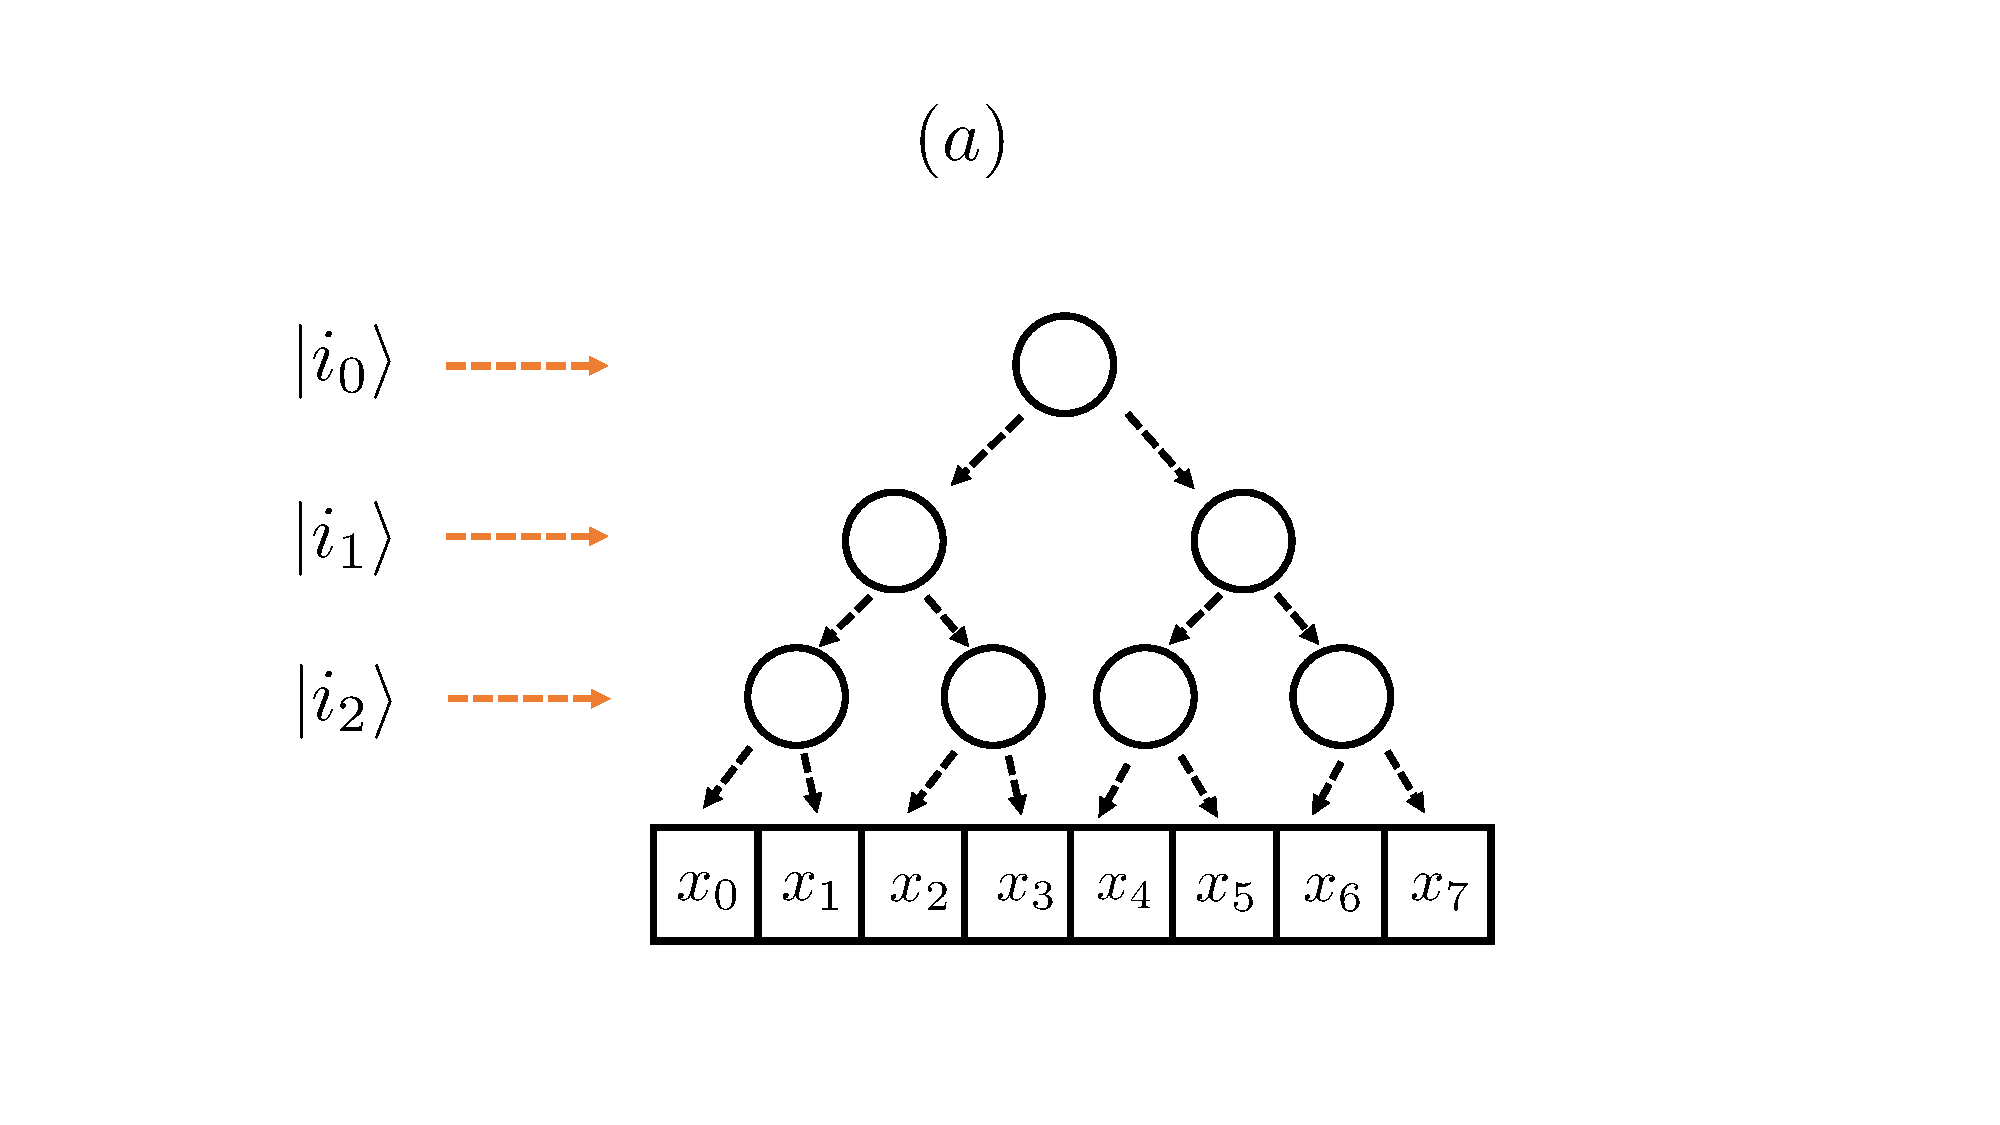
\includegraphics[width=0.45\textwidth]{qram1.pdf}
     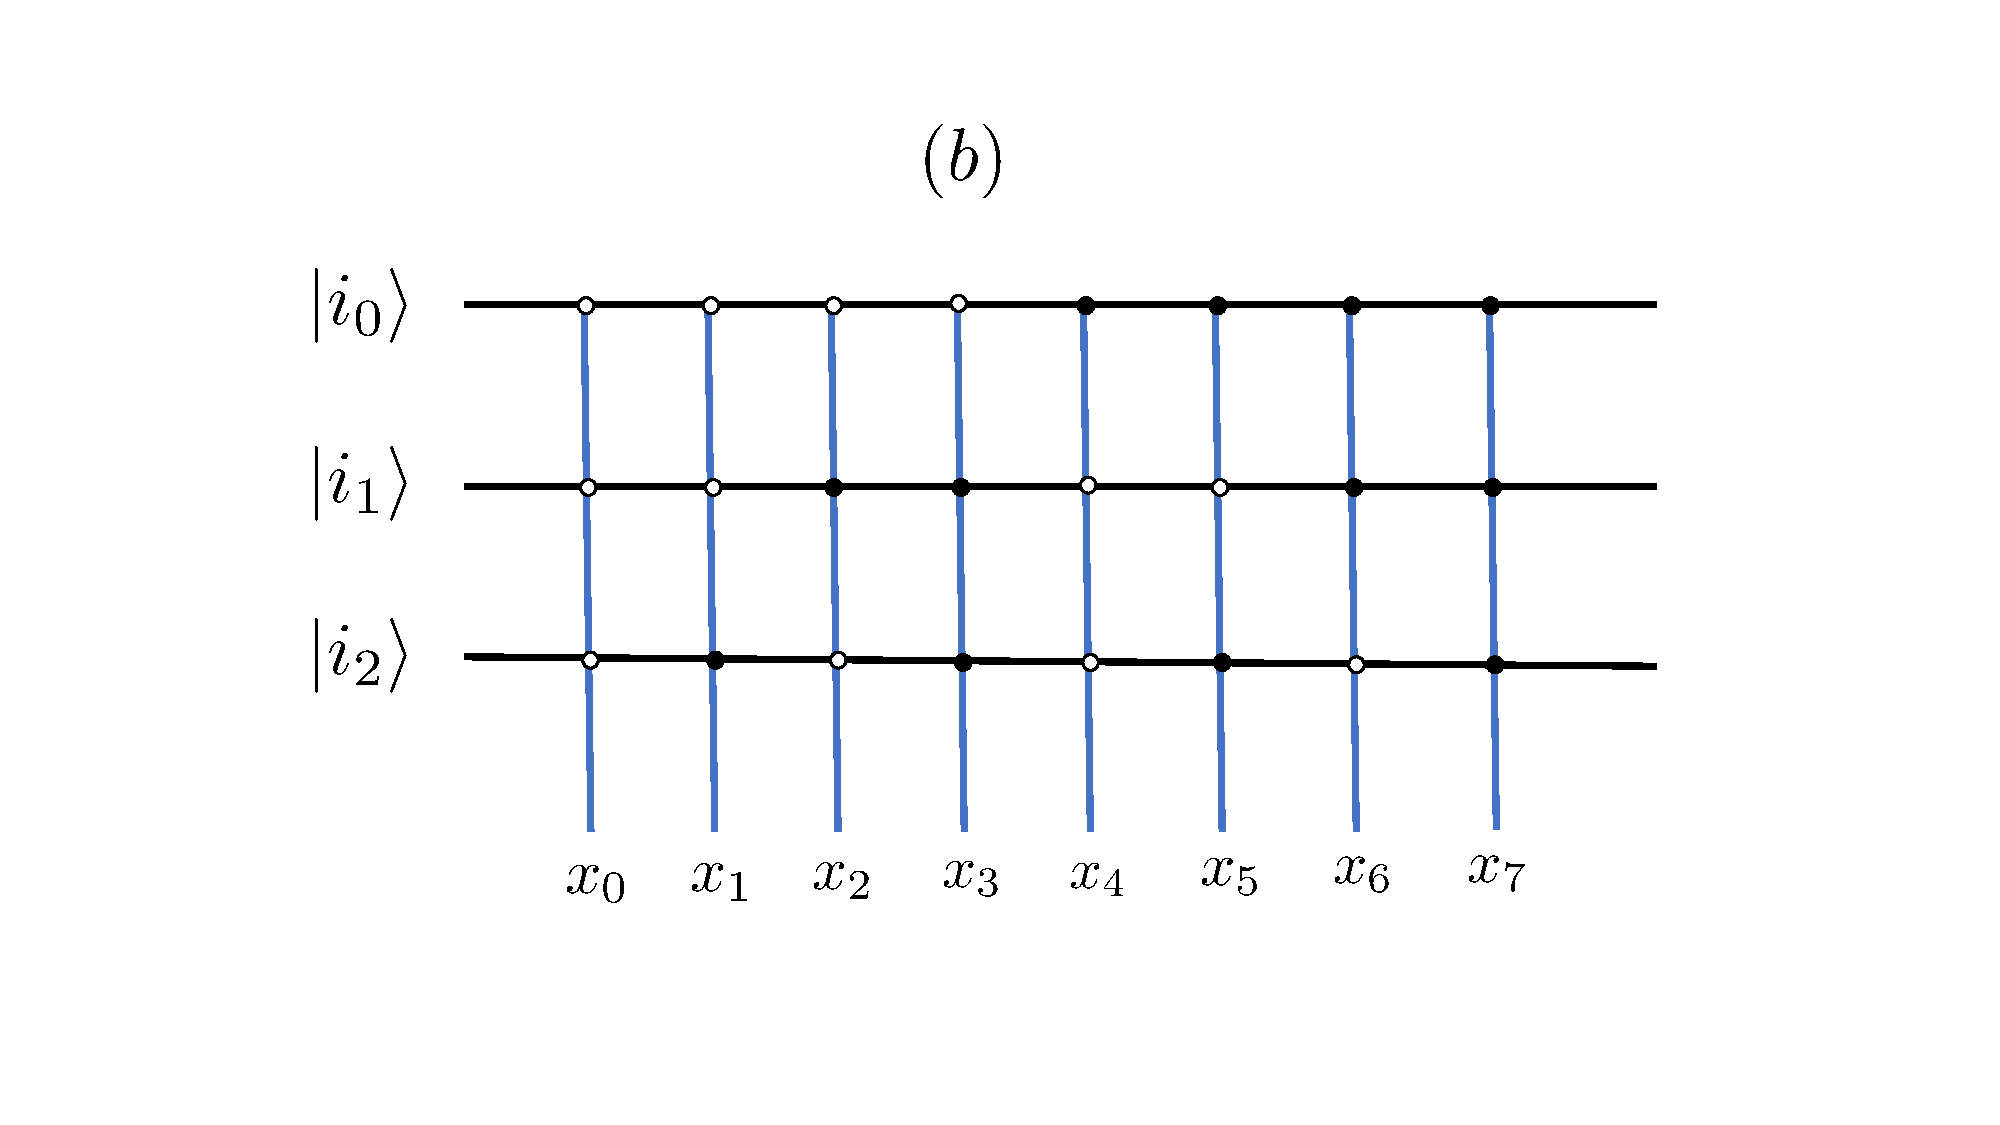
\includegraphics[width=0.45\textwidth]{qram2.pdf}
     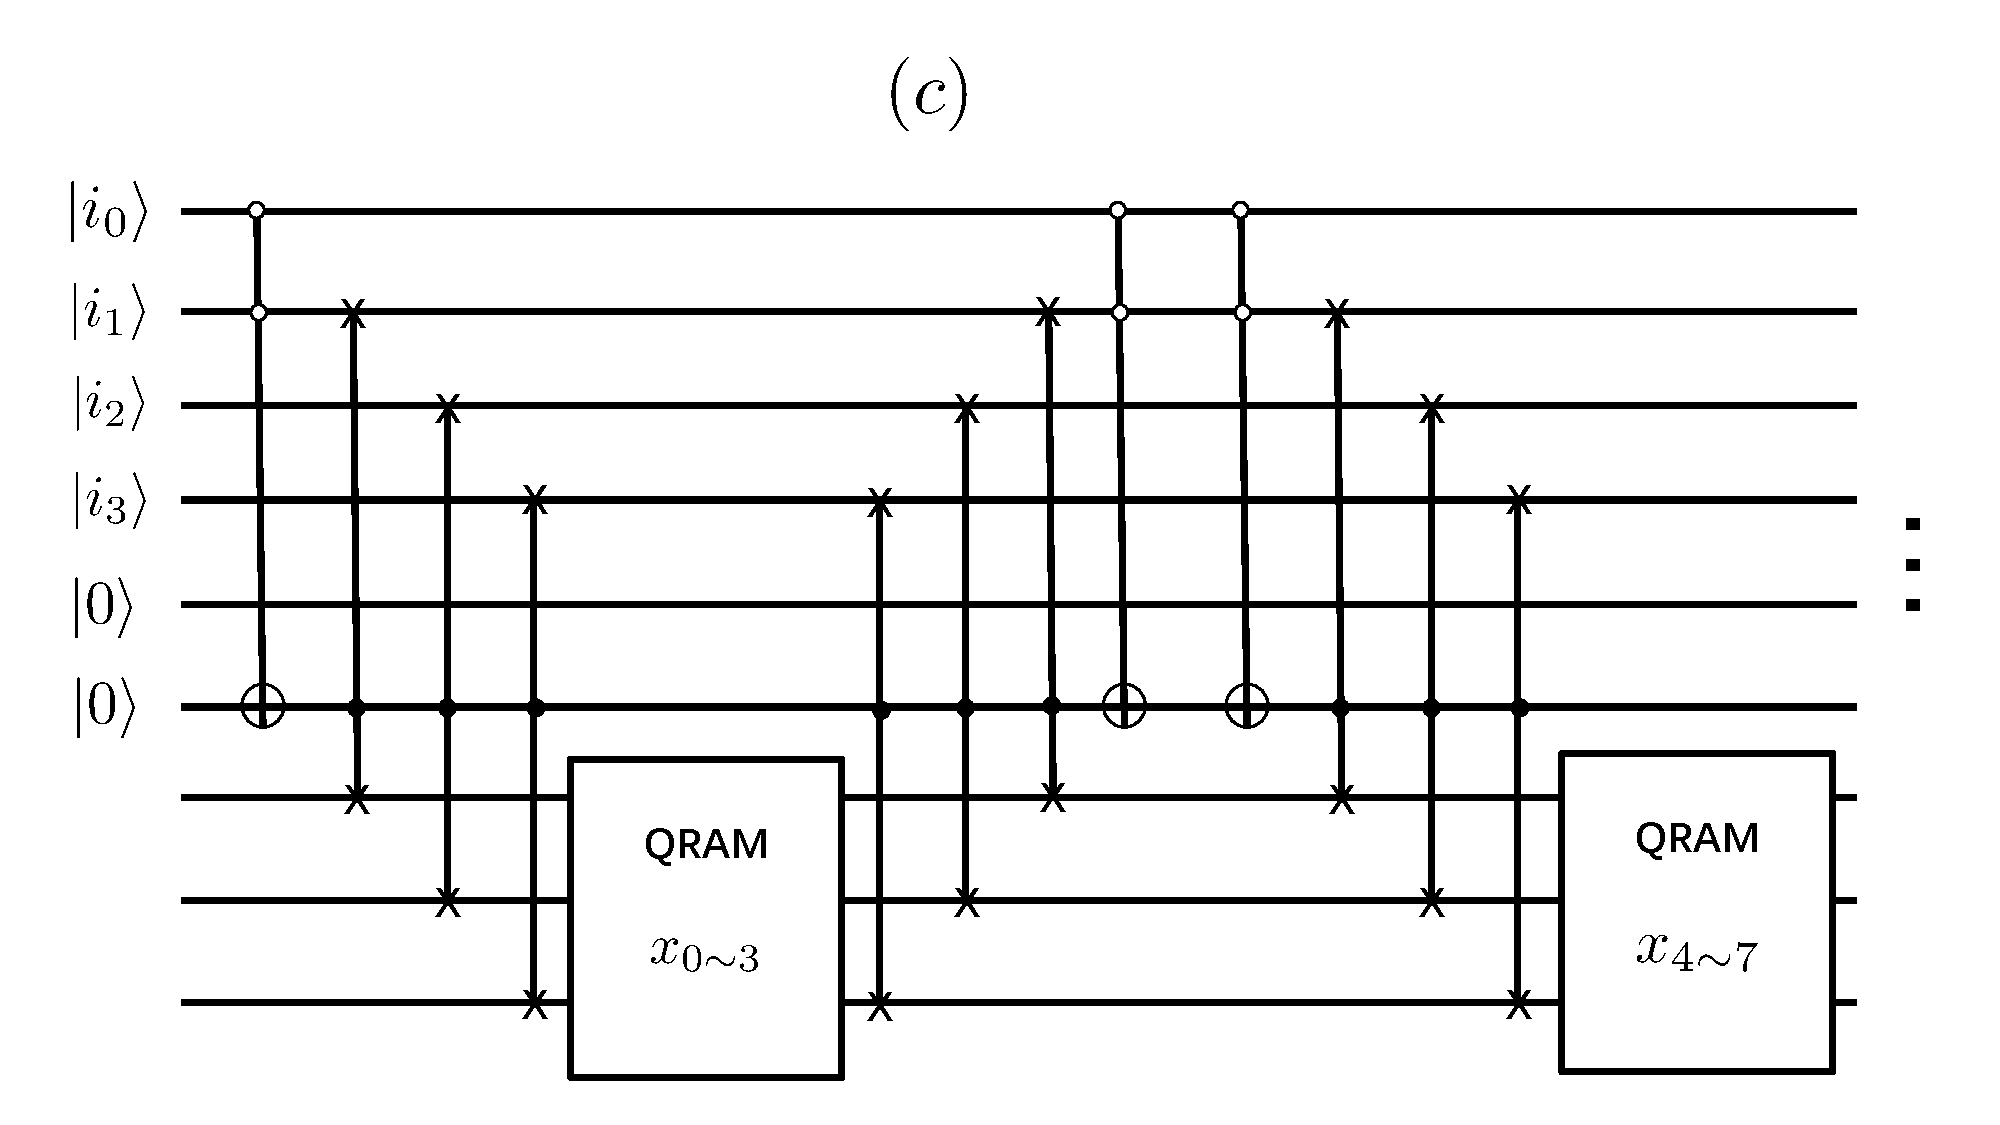
\includegraphics[width=0.6\textwidth]{qram3.pdf}
    \caption{$(a)$ An illustration of QRAM made by quantum routers. $(b)$ An illustration of QROM. $(c)$ Hybrid QRAM-QROM architecture.}
    \label{fig:qram}
\end{figure*}

QRAM might potentially have numerous applications if it is realized on a large scale. Here we summarize some potential applications of QRAM.
\begin{itemize}
\item Quantum algorithms. Many quantum algorithms based on quantum machine learning~\cite{wittek2014quantum,biamonte2017quantum} might require QRAM as a quantum oracle for providing potential exponential quantum speedups. Refs.~\cite{jiang2022quantum,liu2022quantum} discuss how quantum algorithms could provide hardware requirements to QRAM architectures. Ref.~\cite{liu2023data} discusses how QRAM could bring potential enhancement for quantum simulation algorithms in a data center setup. For instance, one could design QRAM circuit for Hamiltonian simulation of quantum chemistry or quantum materials similar to~\cite{babbush2018encoding}, which is an efficient way for uploading Hamiltonian data towards quantum computers. 

\item Quantum data centers. Nowadays, data centers are important businesses in the digital society, and it is natural to have a quantum version of data centers in the coming era. Refs.~\cite{liu2023data,liu2023quantum} propose a theory of quantum data centers (QDCs), where QRAM and quantum networks are combined to provide an elementary definition of QDC. These works show that QDCs with several applications in QRAM as fast quantum memories, will provide fast, secure, and accurate applications in quantum computing, communication, and sensing. 
\item Quantum communication and sensing. Quantum Private Queries~\cite{giovannetti2008queries} and the associated blind quantum computing~\cite{giovannetti2013efficient} could be flagship applications of QRAM in quantum communications, where the users could ask data centers to provide specific services without privacy leakage. Moreover,~\cite{liu2023data} provides a quantum data compression algorithm based on variants of QRAM, an application helpful for distributive quantum sensing applied to, for instance, quantum telescopes~\cite{gottesman2012longer}. 
\end{itemize}

Fault-tolerant designs of quantum random access memory are investigated by~\cite{di2020fault}, showing that QRAM with full fault tolerance might be very challenging on a large scale. However, on the other hand, in~\cite{hann2021resilience}, it is shown that noisy QRAM might still be error-resilient for generic setups of decoherence and noisy channels. In fact, though fanout QRAM designs might be vulnerable to decoherence, rendering them non-scalable, the bucket brigade QRAM architecture is known for its high noise resilience~\cite{giovannetti2008quantum, hann2021resilience}. Specifically, the infidelity of a query grows only logarithmically with memory size~\cite{hann2021resilience}. Yet, past studies leaned on specific noise models, raising questions about the practical advantages in real-world implementations. Ref.~\cite{hann2021resilience} delved into the effects of decoherence on QRAM in a comprehensive manner. A significant takeaway is the affirmation that the logarithmic infidelity scaling persists across varied error channels, including challenges like depolarizing noise and coherent errors. The research identifies limited entanglement among the memory components as the chief reason behind this noise resilience. Interestingly, this insight also suggests potential architectural simplifications without compromising noise resilience, serving an interesting future research question. This understanding implies that with contemporary hardware, QRAM might be potentially realized in real-world noisy environments, facilitating high-fidelity queries even with early fault-tolerant technologies. Additionally, when quantum error correction is integrated, the bucket brigade architecture continues to show promise, enhancing hardware efficiency and fortifying against logical errors~\cite{giovannetti2008quantum, hann2021resilience}.


\paragraph{Experimental efforts towards QRAM: }
Aside from theoretical studies, significant experimental progress has been made towards realizing QRAMs. In one of the original papers on QRAM~\cite{giovannetti2008architectures}, two different fanout designs are presented together with the bucket-brigade designs, quantum optical fanout and phase gate fanout, where hybrid systems of photons and trapped atoms are used. Ref.~\cite{jiang2019experimental} realizes a quantum memory of 105 qubits carried by 210 memory cells in a macroscopic atomic ensemble, with demonstrations of storage of optical qubits into these memory cells and their readout, which might be a significant step towards full quantum random access memory with superpositions of addresses.

Refs.~\cite{hann2019hardware,hann2021resilience,connorthesis} propose a hardware-efficient QRAM design with Hybrid Quantum Acoustic Systems. More precisely,~\cite{hann2019hardware,hann2021resilience,connorthesis} introduce a methodology for quantum computation utilizing multi-modal quantum acoustic systems and, based on this framework, suggest a streamlined approach for QRAM construction. Quantum data is preserved in high-Q phonon modes. Interactions between these modes are deliberately crafted by applying off-resonant stimuli to a transmon qubit. Contrasted with previous suggestions that emphasize direct qubit excitation, it is claimed that their approach can significantly enhance gate fidelity, especially for enduring acoustic modes.

Ref.~\cite{chen2021scalable} introduces a QRAM construction approach using a photonic-integrated-circuit (PIC) architecture combined with solid-state memories. Additionally,~\cite{chen2021scalable} offers a novel scheme rooted in quantum teleportation, further expanding its application in quantum networks. Both of these methods effectively carry out the primary QRAM functions: quantum state transfer and quantum routing. These implementations are grounded in existing components, including electro-optic modulators, a Mach-Zehnder interferometer (MZI) network, and nanocavities linked to artificial atoms for spin-based memory operations.

Constructing a large-scale, fault-tolerant QRAM presents significant challenges, which could be summarized as the following.
\begin{itemize}
\item Scalability: The number of qubits required for a QRAM scales linearly with the data set size. As data sets grow, so does the qubit demand. Moreover, larger data sets necessitate more substantial QRAM hardware with higher circuit depth and more sophisticated designs.

There are various ways to address the scalability issue by hardware co-designs of QRAM. For instance, we can utilize $\text{Q}^2$ routers as foundational components for constructing QRAM (Here, $\text{Q}^2$ router refers to the router with both control and signal states being quantum states). This modular design allows us to assemble QRAM by interlinking various modules, as depicted in Figure \ref{fig:challenges}. Alternatively, a 2-D integrated QRAM can be achieved using \emph{H-tree} patterns, either through the teleportation protocol as outlined in~\cite{xu2023systems} or by employing long wires (see Figure \ref{fig:challenges2}. Note that this design is beyond~\cite{xu2023systems} by implementing long-range coupling wires, within the capability of IBM devices. Moreover, the design is compatible with a \emph{single-layer} architecture without crossing coupling wires). For a scalable QRAM, extensive range connectivity might be bounded by some principles of physics as discussed in~\cite{wang2023fundamental}. 

\item Efficiency: To ensure QRAM's efficiency and reliability, the quantum hardware must be both highly compact (fractal or self-similar structures in the design of QRAM with more efficient usages of space like~\cite{xu2023systems}) and highly coherent. In addition to superconducting circuits, it is also intriguing to explore more compact phononic circuits for QRAM like~\cite{hann2019hardware}.

\item Error Correction: As QRAM size expands, errors become inevitable. Thus, strategies for reliable data loading despite these errors are essential. Standard quantum error correcting codes might be applicable to QRAM. However, developing quantum error correction techniques that are specifically adapted to QRAM~\cite{di2020fault,jaques2023qram} remains an open research area. On the other hand, error resilience of designs of QRAM~\cite{hann2021resilience} might provide possible resolutions. Moreover, error resilience is a feature of bucket-brigade QRAM, which shows that errors only scale poly-logarithmically with the system size (see above). This indicates that QRAM can already be a useful application for some non-error-corrected quantum computers.

\item Need for Specialized Solutions: Given its unique purpose and architecture, QRAM's scalability issues should be approached with its specific needs in mind. Unlike universal quantum computers, QRAM doesn't need a universal set of quantum operations, which could be an avenue for simplifying its architecture. Moreover, some classical optimization could be helpful to enable more sophisticated QRAM designs. For instance,~\cite{hann2021resilience} designs a noisy QRAM simulator in classical devices, which might be for further explorations of QRAM designs and simulation in a classical space. 



\end{itemize}


\begin{figure*}
    \centering
     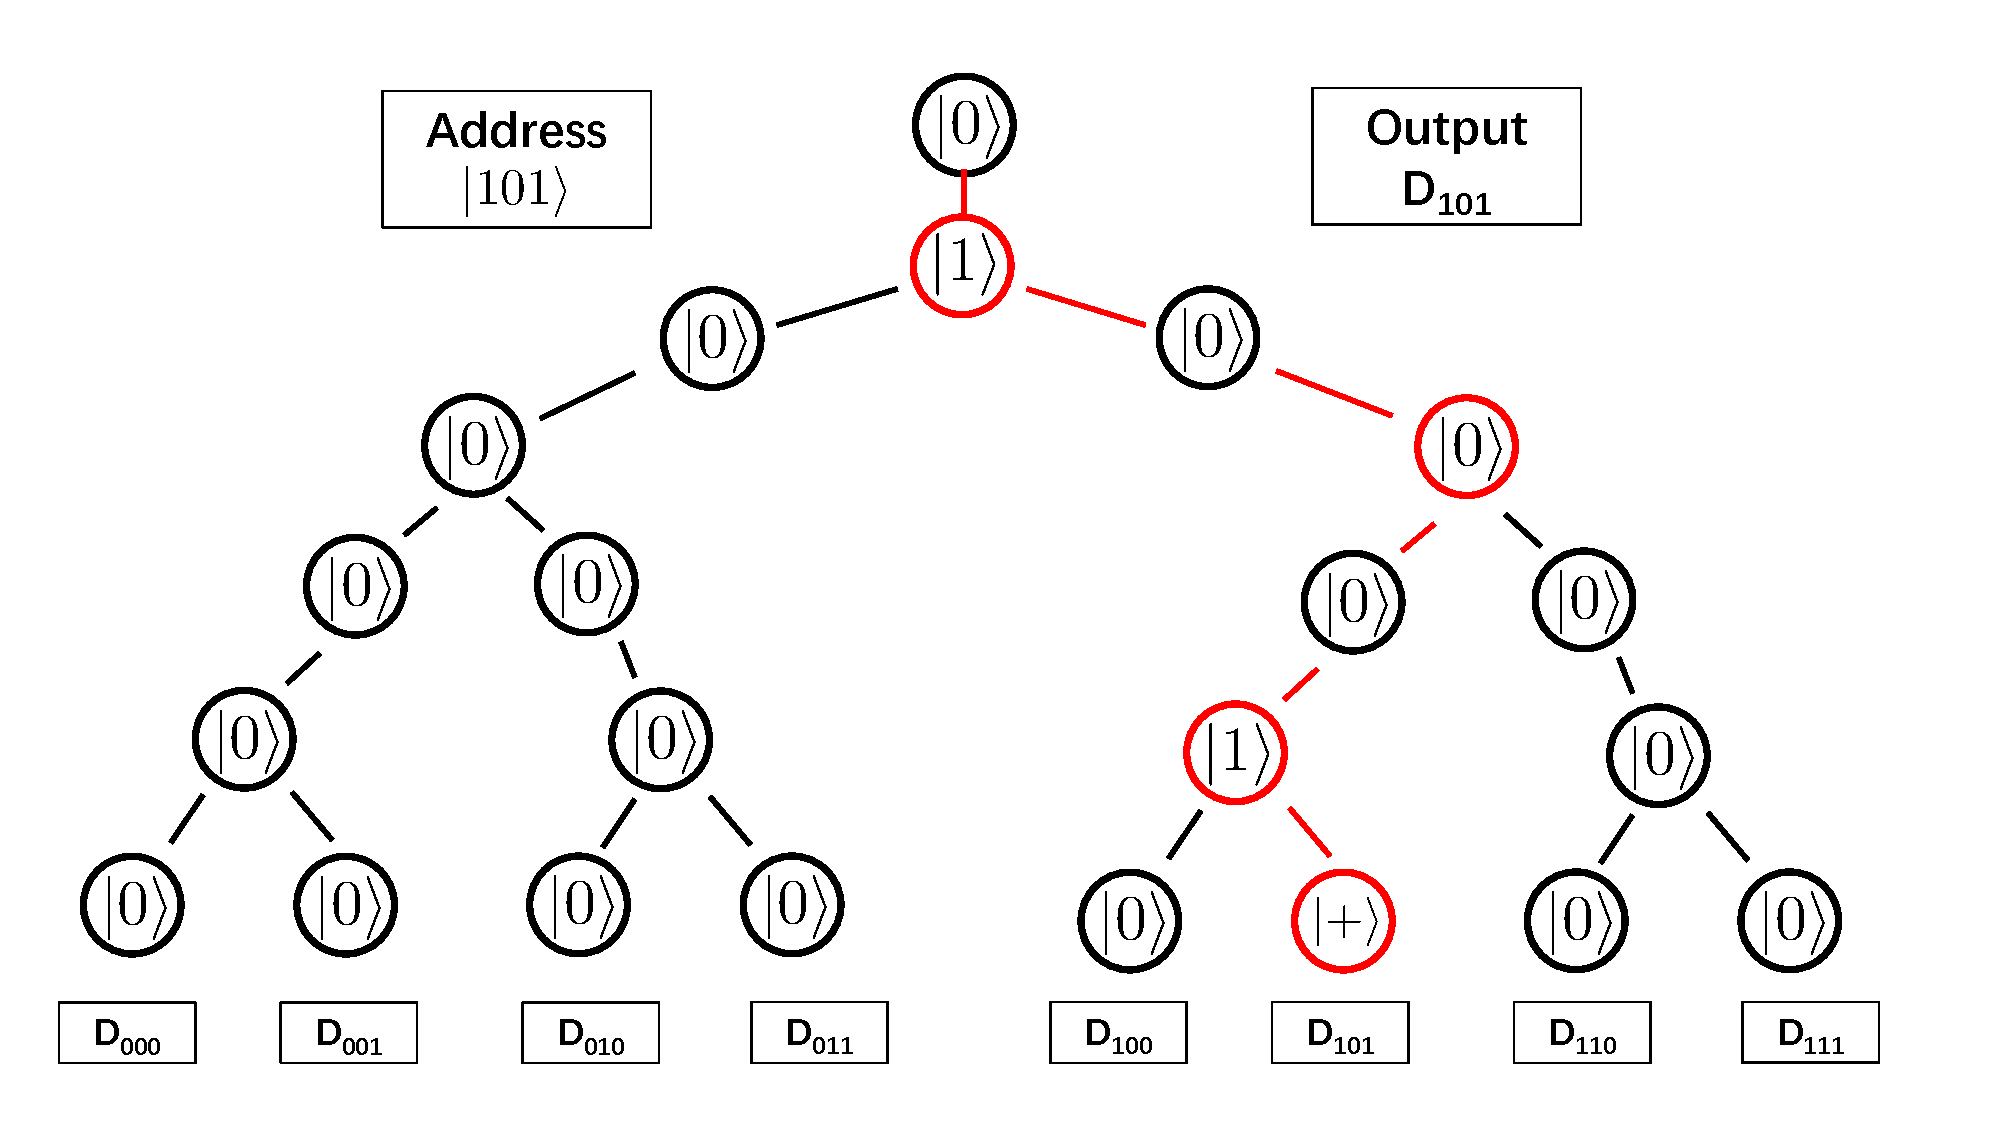
\includegraphics[width=0.6\textwidth]{qram4.pdf}
     \caption{QRAM as a binary tree of $\text{Q}^2$ routers. Here, $\text{Q}^2$ router refers to the router with both control and signal states being quantum states.}
     \label{fig:challenges}
\end{figure*}

\begin{figure*}
    \centering
    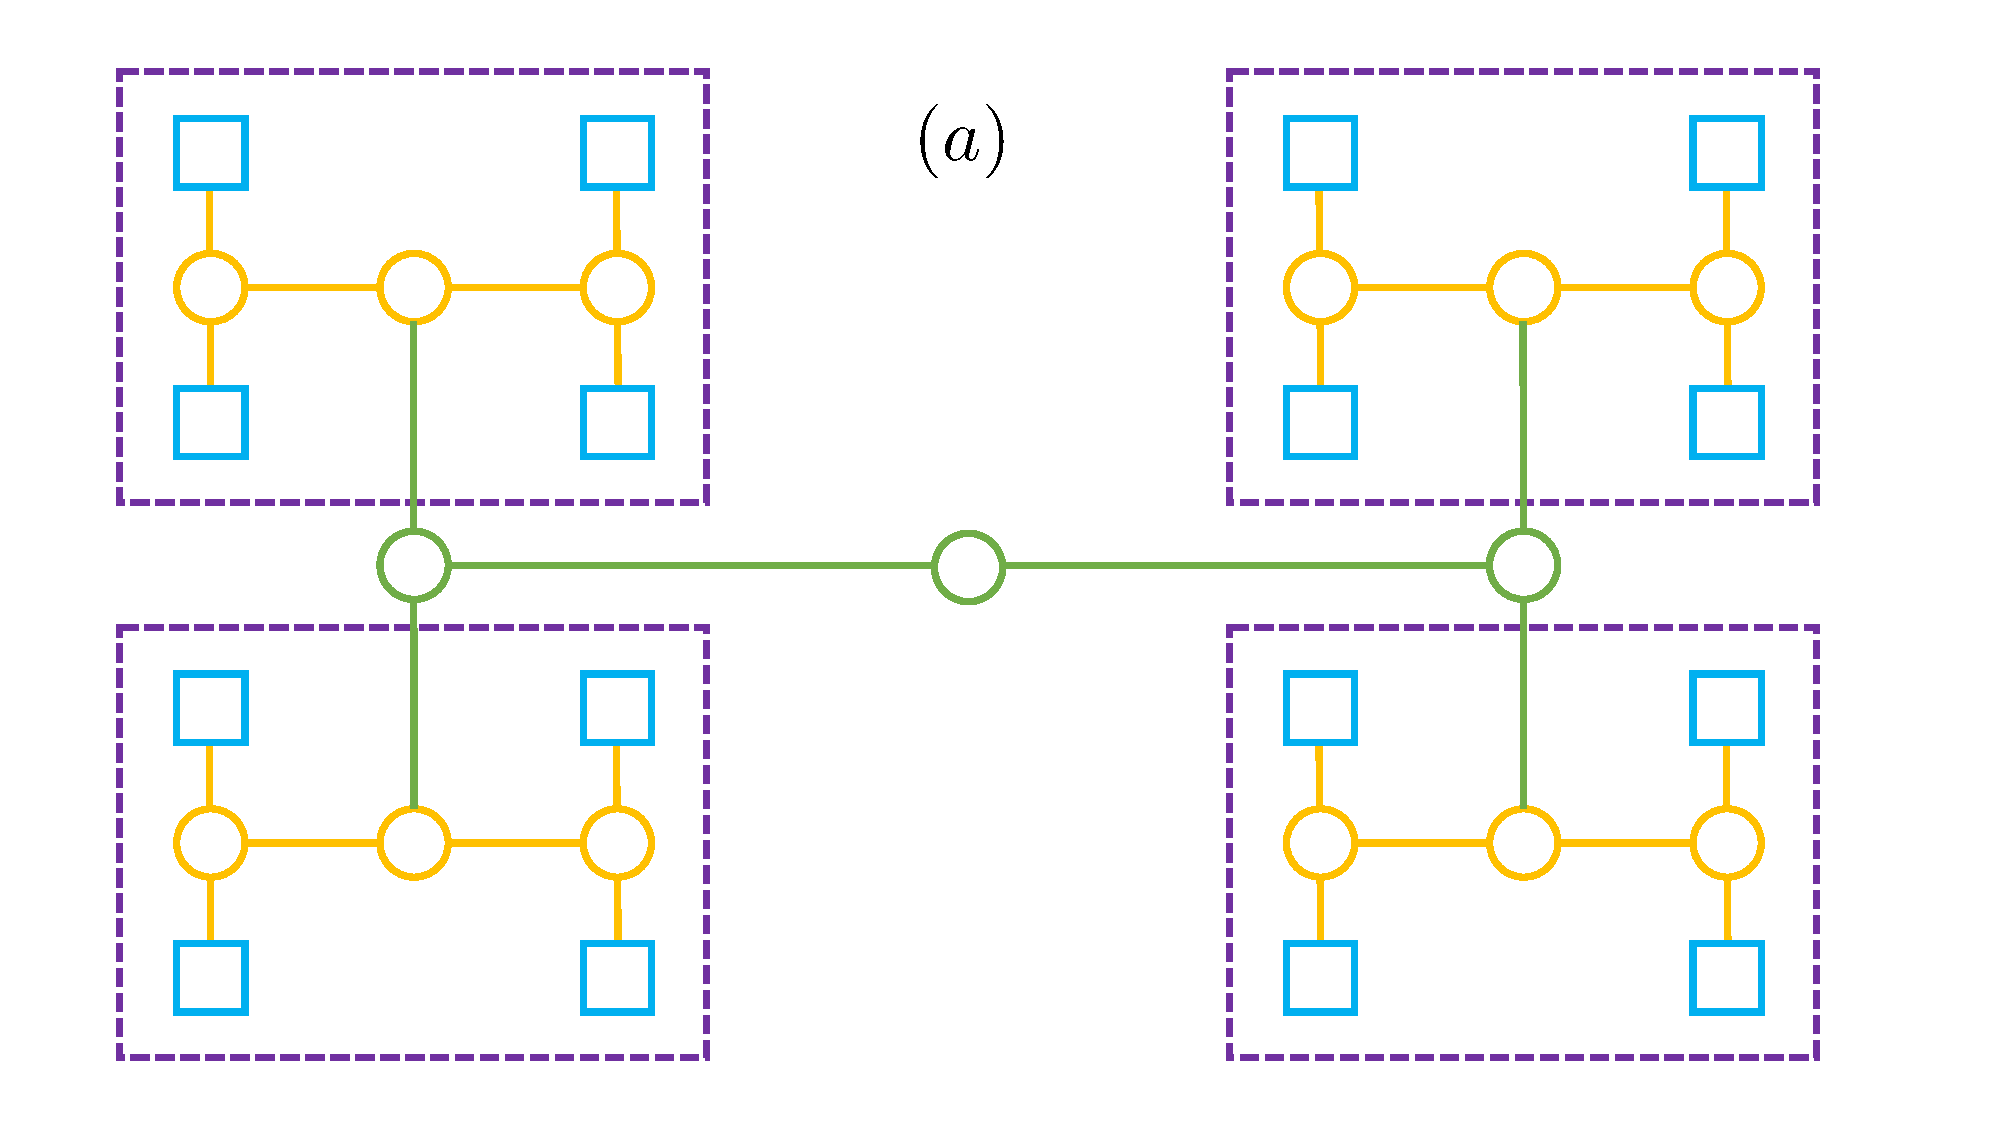
\includegraphics[width=0.45\textwidth]{qram6.pdf}
     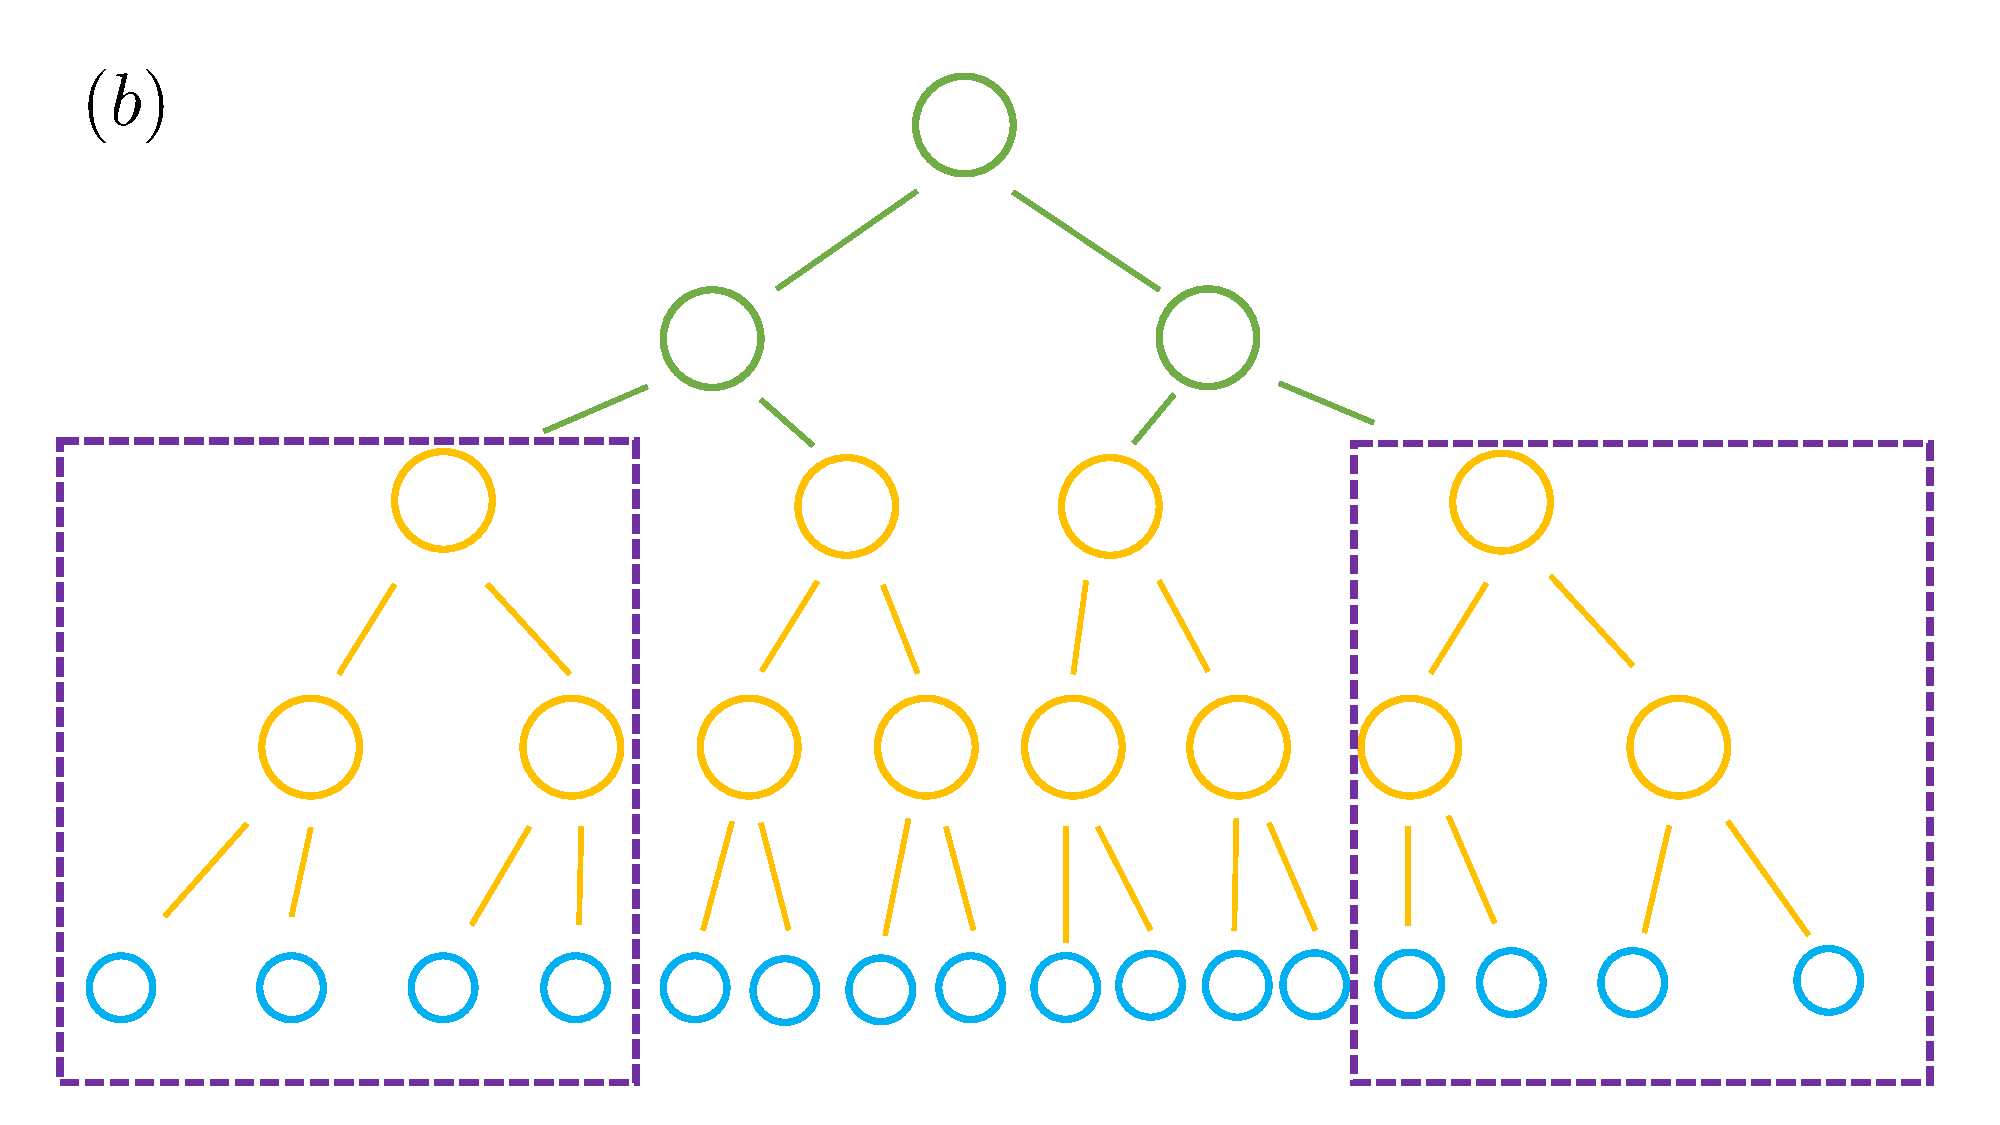
\includegraphics[width=0.45\textwidth]{qram7.pdf}
     \caption{$(a)$ Self-similar fractal structure of the H-tree designs (see~\cite{xu2023systems}). One can use the self-similar structure to create a size $2^{n+2}$ QRAM from 4 units of size $2^n$ QRAM. $(b)$: An example of depth-4 tree with $2^4=16$ leaves. }
     \label{fig:challenges2}
\end{figure*}



\subsection{Circuits, transpilation, and architecture}

Just as in classical computing, every quantum computation that is to be carried out on a quantum computer needs to be broken down to a netlist of native operations that admit a direct implementation on a quantum computer. One of the most widely-used representation of such a netlist is the so-called quantum circuit, which is to be transpiled for a target quantum computer backend. Different quantum hardware backend may support different qubit-to-qubit connectivity, which limits the interactions between the qubits that may be implemented natively. 

To this end, quantum applications in materials science are no exceptions. Indeed, quantum circuits for Heisenberg hamiltonian simulation~\cite{childs2018toward,nam2019low}, relevant for many-body localization and room-temperature superconductivity, and electronic structure calculations for small molecules~\cite{nam2020trappedion,wang2021resource,wang2023ever}, relevant for chemical reactions, have been optimized for both pre-fault tolerant and fault-tolerant settings before. Other examples include particle physics simulations~\cite{shaw2020quantum,kan2021lattice,kan2022simulating}, where fault-tolerant cost, including the number of non-Clifford quantum gates and qubit counts, have been minimized. In all these examples, it is critical that the resulting netlist of instructions to be carried out by a quantum computer is optimized, targeting {\it time to solution}: It is a key metric in all types of computation, including quantum. Case in point, if time to solution is of no matter, the computational advantages offered by quantum computing is moot and classical computing suffices, and a high-fidelity operation of a quantum computer would become unnecessary since repeated executions of computation can be performed until a correct answer is obtained. The important roles that circuits, transpilation, and architecture will continue to play in leveraging the computational power enabled by quantum computation then form the central topics of this section.

\subsubsection{Connectivity and Architecture}
\label{sec:CNA}

We begin by highlighting key topics around qubit connectivity, a fundamental aspect of QPUs that dictates the efficiency, scalability, and feasibility of the quantum devices. We first consider SWAP networks, highlighting their role in enabling Hamiltonian simulation in quantum systems with limited connectivity. The discussion then moves to distributed quantum computing, emphasizing its importance in scaling quantum computing beyond the capabilities of current QPUs. Quantum circuit cutting is also examined for its practicality in decomposing complex quantum circuits into smaller segments, facilitating distributed processing.


\paragraph{SWAP networks} One of the tools that can be leveraged to effectively implement Hamiltonian simulation primitives on hardware with minimal (linear) connectivity is the SWAP network~\cite{kivlichan2018quantum, tomesh2021coreset,hashim2022optimized}. Through a SWAP network (depicted in Figure~\ref{fig:swap_network}), all $\binom{n}{2} \in O(n^2)$ pairs of (commuting) interactions between $n$ qubits can be accomplished in just $O(n)$ circuit layers, even on a quantum computer architecture that admits nearest-neighbor qubit-to-qubit connectivity. With the exception of an all-to-all architecture that admits a single-instruction implementation of commuting, overlapping two-qubit gates~\cite{grzesiak2020efficient,grzesiak2022efficient,bravyi2022constant}, the asymptotic scaling of $O(n)$ matches that admitted by an architecture that allows for random-access two-qubit interactions that may be implemented in parallel so long as the interactions do not overlap. In the context of the Materials Science applications in this paper, any ``dense'' interactions with commuting terms can have a natural implementation on an all-to-all architecture (c.f. Refs.~\cite{nam2019low,wang2021resource,kan2022simulating,wang2023ever}) or on a limited-connectivity architecture with SWAP networks. Reducing the overhead in moving the quantum information around for optimal implementation of a given set of two-qubit interactions remains an area of ongoing research.

\begin{figure}[htbp]
    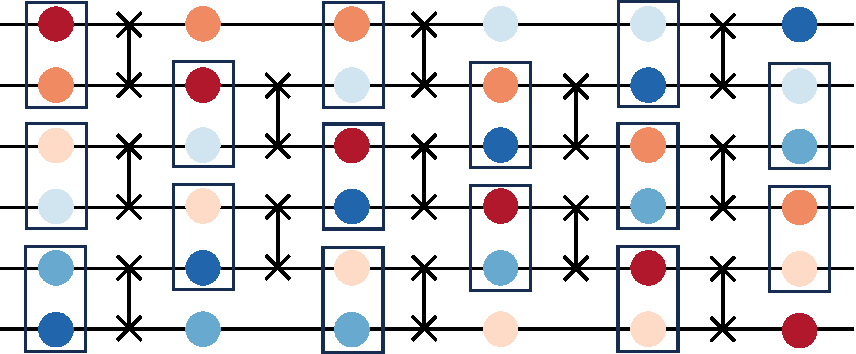
\includegraphics[width=\linewidth]{figures/SWAPNetwork.pdf}
    \caption{Example SWAP network for $n=6$ qubits. In $O(n)$ steps, each of the $O(n^2)$ pair of qubits (colors) performs an interaction, even with just linear connectivity.}
    \label{fig:swap_network}
\end{figure}


\paragraph{Distributed/modular}
Just like classical HPC, distributed quantum computing is necessary for the continued scaling of quantum computing. While monolithic quantum processing units (QPUs) continue to make significant progress in both sizes and qubit qualities, there remains a huge gap between available QPUs and practical benchmarks. To make matters worse, developments from classical computing demonstrate that the computing and memory capacity gaps between large-scale industrial use cases and single computing cores only get larger, despite having more powerful monolithic cores. To combat this increasing gap, almost all industry-scale classical applications today such as Large Language Model (LLM) training, and even many personal-scale workloads such as intensive gaming, happen in parallel. In fact, distributed computing is only more imperative for quantum computing as single-core scalability poses significant engineering challenges.

There have been distributed quantum computing proposals from both hardware and software researchers. IBM, Quantinuum, and IonQ all announced plans to develop modular QPUs with interconnects to enable distributed quantum computing.
Ref.~\cite{ang2022architectures} models hardware performances of potential superconducting modular QPUs.
Ref.~\cite{wu2022collcomm} proposes compilation algorithms for distributed QPUs with EPR pair connections. 
Ref.~\cite{Zhang_2022} proposes ClusterVQE which enables domain-specific optimizations to map applications from a target domain (here, variational quantum algorithms) to distributed QPUs.
Further research across the stack from applications to devices is necessary to enable distributed quantum computing with tolerable overheads.

\paragraph{Circuit cutting}
Quantum circuit cutting offers an orthogonal software path to enable distributed quantum computing to hardware modular QPUs. Cutting qubit wires~\cite{peng2020simulating} or quantum gates~\cite{piveteau2023circuit} breaks down a large quantum circuit into multiple smaller subcircuits. Multiple less powerful QPUs run the smaller subcircuits in parallel. Classical computing eventually reconstructs the original circuit output. End-to-end implementations~\cite{tang2021cutqc, tang2022scaleqc} demonstrate cutting up to $200$-qubit benchmarks to distribute onto multiple QPUs available nowadays, which are otherwise intractable for purely quantum computing or classical simulations. The primary challenges in applying quantum circuit cutting at practical scales stem from the demands of classical post-processing: firstly, the output length of an n-qubit circuit is $2^n$, which rapidly strains classical memory and processing time for large quantum circuits; secondly, the classical post-processing effort scales exponentially with the number of required cuts, $K$, further constraining the runtime.

Despite its ability to run previously intractable workloads, there is still a gap between the computational capacity of circuit cutting now and future practical quantum workloads. The first theory proof~\cite{peng2020simulating} proposed an exponential classical reconstruction cost. Instead, subsequent works~\cite{tang2022scaleqc} drastically reduce the overhead to sub-exponential but remain prohibitive in the worst case. Filling the gap calls for further developments in classical reconstruction techniques, algorithm-backend co-design, and quantum computing cloud backend system adaptations~\cite{serverless}.

In the next two paragraphs, we shift attention to elements beyond QPUs, addressing key developments in memory and qubit-state storage. We delve into QRAM and QROM, emphasizing how compiler strategies like the Gray Code can enhance memory efficiency. Further, we examine multimode cavity systems, an innovation in quantum memory, providing effective storage solutions for qubit states while also introducing distinctive integration and scalability challenges. How these memory elements are to be eventually integrated with a to-be-developed compiler to enable efficient quantum computing is an open area of research.


The QRAM and QROM memory primitives discussed earlier can be optimally implemented with appropriate compiler techniques. As one example, consider the Gray Code, a sequence of the $2^n$ n-bit bitstrings such that only 1 bit changes between sequential neighbors, for instance, 000, 001, 011, 010, 110, 111, 101, 100. Integrating awareness of the Gray Code in a compiler can significantly reduce gate counts for memory implementations. Additional compilation techniques for these memory primitives, including routing and mapping, are discussed in prior work~\cite{di2021improving, xu2023systems,wang2023fundamental}.


Multimode cavities with tens of modes and photon lifetimes on the order of milliseconds pose as efficient mediums to store multiple qubit states. When used as quantum memory or registers, they can allow for effectively extending the lifetimes of qubits. These cavities can be coupled with one physical qubit, to allow for swapping of a qubit state in and out of the cavity to perform multi-qubit operations with other qubits. 
While integrating multimode cavities reduces swap-distance to enable multi-qubit gates for a larger number of qubits, it also imposes serialization of swaps of qubit states from a single cavity posing additional compilation challenges. In terms of physical integration of these cavities to superconducting circuits, there remain challenges in terms of reducing 3D-cavity size or utilizing 2D resonators while maintaining long lifetimes of stored qubits~\cite{chakram2021seamless}.


\subsubsection{Circuit optimization}
\label{sec:Circ}
\paragraph{Sequences of Pauli rotations} Most standard implementations of Hamiltonian propagators rely on the implementation of a sequence of Pauli rotations, often coming from a Trotter expansion.
In the near-term setting, a sequence $R_{P_k}(\theta_k)\cdots R_{P_1}(\theta_1)$ is usually implemented via an alternating sequence of Clifford circuits and single-qubit rotations.
This prompts the natural problem of finding the best possible sequence of interleaved Clifford circuits and single-qubit layers implementing some goal sequence of Pauli rotations.
In some cases, the ordering of the rotations may also be relaxed, leading to even further optimizations.
Some work already tackles this synthesis problem both for all-to-all architectures and for restricted coupling maps~\cite{childs2018toward,nam2019low,nam2020trappedion,cowtan2020generic,wang2021resource, li2021software, martiel2022architecture,wang2023ever}.
This problem is tightly related to the \emph{parity network synthesis problem} introduced in~\cite{amy2018controlled}, for which many architecture-aware heuristics have been developed~\cite{vandaele2022phase,meijer2020architecture}. It is still an open question to formalize the notion of Pauli networks in the presence of ancillas and measurements. 

\begin{figure*}
    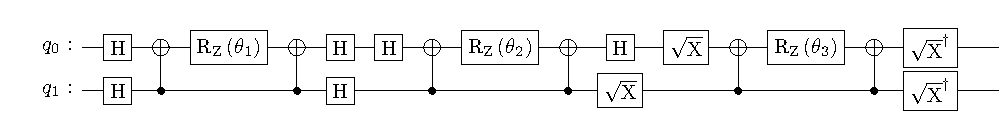
\includegraphics[width=0.45\textwidth]{figures/pauli_rotations_bad.pdf}\\
    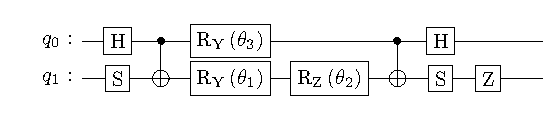
\includegraphics[width=0.45\textwidth]{figures/pauli_rotations_good.pdf}
    \caption{Two circuits implementing the same sequence $R_{\operatorname{YY}}(\theta_3)\cdot R_{\operatorname{XZ}}(\theta_2)\cdot R_{\operatorname{XX}}(\theta_1)$.}
    \label{fig:enter-label}
\end{figure*}

\paragraph{Feedforward} One of the key emerging tools for efficient compilation is dynamic circuits that make mid-circuit measurements that feedforward into subsequent operations. While in principle any quantum circuit can be implemented without midcircuit measurements, due to the \textit{principle of deferred measurement}, there are several scenarios where the dynamic approach significantly lowers circuit depth or circumvents topology constraints. For example, controlled rotation gates can be implemented with a smaller number of non-Clifford gates using feedforward~\cite{jones87novel,nam2020approximate}, which are beneficial for optimizing Heisenberg hamiltonian simulations~\cite{nam2019low}. Another example may be that, while a $n$-qubit GHZ state requires $O(n)$ layers with linear qubit connectivity (and $O(\log n)$ layers with all-to-all connectivity), the state can be produced in constant $O(1)$ depth with feedforward midcircuit measurements. More generally, any Clifford circuit can also be implemented in constant depth with midcircuit measurements on linear nearest-neighbor connectivity. In the context of materials science applications, this is useful for primitives such as the CNOT ladder used in Hamiltonian simulation. Provided with the already identified utility of feedforward in optimizing quantum circuits, further developments in the use of feedforward to optimize additional elements of quantum circuits are anticipated.

\paragraph{Pre-fault tolerant vs. Fault-tolerant} The central task of a compiler is to translate a human-readable code to a machine code that can then be executed by a computer using its native operations. As such, the compiler plays a critical role in both the accessibility of the software development environment for the end users and the efficiency of the machine code that faithfully implements the code that the users want to execute using the least amount of computational resources. Specifically to the latter, an optimizing compiler can be developed, which takes into account various computational operations, possibly having varying cost~\cite{nam2018automated,nam2019low,wang2021resource}. An example applicable to quantum computing may be in the context of the pre-fault tolerant vs. fault-tolerant quantum computers, where the former typically enjoys faster and higher-fidelity single-qubit operations compared to entangling operations, whereas the latter admits significantly less expensive implementations of Clifford operations over non-Clifford counterparts, e.g., single-qubit T gates. A powerful compiler would then enable an end user to develop quantum software at ease -- hopefully in most cases independent of the backend details -- while behind-the-scenes custom-optimizing for different backend quantum computer hardware, including the availability of fault tolerance.

\paragraph{Approximate compilation} Oftentimes, the freedom to implement target unitaries only \textit{approximately} is a powerful tool that can lead to significant cost reductions. For example, this technique has enabled improvements in quantum volume~\cite{cross2019validating}, qudit SWAP gates~\cite{campbell2023superstaq}, bosonic interactions~\cite{shaw2020quantum,kan2021lattice,kan2022simulating}, and even the leading proposal for Shor's Algorithm~\cite{gidney2021factor}, in which exact addition is replaced by approximate addition. Indeed, the widely-used quantum Fourier transform is also implemented approximately in practice~\cite{coppersmith2002approximate,nam2018automated}, and in most quantum simulation algorithms an integral component is implementing a time evolution operator approximately. Beyond approximating unitaries, approximate compilation has also been employed in conjunction with knowledge of the input state, where one quantum circuit may be replaced with another as long as their actions on the input state is similar (even if the actions on some other states might be different). Given the important role that approximate methods play in classical computing -- consider for example numerical integrators or polynomial-time approximation scheme for NP-hard or \texttt{\#}P-complete problems -- fruitful research outcomes that leverage approximate compilation, broadly defined, are expected. Adding to the flavors of approximate compilation research works mentioned earlier, possible, non-limiting research avenues may include (c.f.~\cite{campbell2019applying,pabst2022quantum,shaydulin2023evidence,dalzell2023quantum} and references therein) continuing to quantify existing approximate methods in classical computing for a speed up (e.g., Grover-like or potentially more) or finding entirely novel approximation schemes for those problems known to be hard to solve for quantum computers (e.g., QMA-complete).

\subsection{Real-time classical processing of quantum information (within coherence time)}
\label{realtimeQuantumClassical}


% Ang Li: 
In this model of hybrid computation, the classical part is embedded or coupled with the quantum program and runs simultaneously with the quantum operations within the coherence time.
This can significantly reduce the data-movement between the classical and quantum processors while providing the desired flexibility and short timing in controlling the quantum state.
With mid-circuit measurement~\cite{corcoles2021exploiting, govia2022randomized}, classical computation can use previous quantum operation outcomes to profile the quantum execution status, predict and even adjust the quantum operations for future iterations or steps.
Some examples are QEC~\cite{brown2023advances}, progressive projection filtering~\cite{ge2019faster, stetcu2023projection} and random walk phase estimation~\cite{granade2022using}.
The key point is that the classical computation has to be performed while the quantum state is still coherent.
Given the short coherence time for near-term devices, constraints on the latency of the classical computation can be stringent, possibly demanding a strongly coupled classical hardware accelerator (e.g., FPGA, GPU, or ASIC) physically in place where classical control is happening.

\subsection{Error mitigation}

The output of quantum devices is inevitably affected by noise. While QEC can theoretically be used to remove error from any computation once error rates of the physical devices are pushed below the fault-tolerance threshold, in the near term various techniques can be used to reduce the effect of noise on computation, generally referred to as quantum error mitigation (QEM)~\cite{kandala2019errormitigation,maksymov2023enhancing,cai2023quantum, stein2023q}. When a noisy quantum device is used to compute expectation values of quantum observables, this in general results in a biased estimator. The goal of QEM is to minimize the bias and variance in expectation values from several different runs of the noisy quantum circuit using classical post-processing.

One method that can in principle recover the ideal noiseless expectation values is probabilistic error cancellation (PEC)~\cite{vanderberg2023probabilistic}.
PEC is based on the inversion of a learned noise model of the device through sampling from a distribution of noisy circuits related to the noise model.
One can prove that the bias of the resulting estimator vanishes as the quality of the learned noise model improves (provided the noise does not change between the noise learning and the actual experiment), but the sampling overhead is exponential in the size of the circuit, with the base of the exponential being related to the noise rate.
While PEC becomes challenging for larger experiments, various techniques can mitigate its cost such as the use of tensor-network-based post-processing \cite{filippov2023scalable} instead of the circuit sampling, which reduces the sampling overhead quadratically, at the cost of more classical computational power. Moreover, the sampling overhead can be contained by improving the accuracy in estimating the noise factors.

An alternative approach to QEM is called zero-noise extrapolation (ZNE). ZNE is based on the collection of noisy expectation values for various amplified values of the noise parameter.
The expectation value at the zero-noise level is then extrapolated using a linear, polynomial, or exponential fit.
ZNE can be implemented using analog (relying on pulse stretching~\cite{kim2023scalable}) or digital amplification methods (such as sub-circuit repetition~\cite{shehab2019toward,giurgicatiron2020digital,majumdar2023best}) that do not require a precise characterization of the noise, or using probabilistic error amplification (PEA) \cite{kim2023evidence}, which achieves the desired noise factor by randomly drawing circuits from a distribution implementing a rescaled Pauli noise model learned from the device.
ZNE does not suffer from the severe sampling overhead of PEC, but it does not produce a guaranteed unbiased estimator.
Its success depends on a proper choice of the fitting method (methods for systematically choosing the most appropriate one have been proposed, e.g.,~\cite{majumdar2023best}), amplification factors for the noise (e.g., too large amplification will destroy the signal, too small amplification will make the extrapolation less precise), as well as the amplification method itself. Recently, ZNE has also been extended to quantum error correction~\cite{wahl2023zero}.

One more technique to boost quantum fidelity through post-processing is Quancorde~\cite{ravi2022boosting}, which uses Clifford ``canary circuits'' (which are classically simulable but also resemble the target application structure and thus suffer similar structural noise impact) to order an ensemble of devices or qubits/mappings approximately along the direction of increasing fidelity of the target application.
One then estimates the correlation of measurement outcome probabilities with this ordering and uses this correlation to weight the noisy probability distribution; correct measurement outcomes are expected to have a higher correlation with the ensemble order, and thus their probabilities are boosted, while those of incorrect outcomes are suppressed. 


QEM has become an integral part of quantum simulations with near-term devices and, together with the constant improvement of the hardware, has allowed for impressive experiments reaching the boundary of what is computable using brute-force classical calculations~\cite{kim2023evidence}.
It will enable us to push the capabilities of the upcoming generations of hardware up to the transition to fault-tolerance, where it can still complement QEC for various use cases.
One potential avenue towards increasing the effectiveness of QEM is to develop either applications that are well-adapted to certain types of error mitigation, or mitigation techniques that exploit information about the specific application.
